\newpage

\section{Konzept}
In diesem Abschnitt wird das Konzept der evaluierten Lösungsvariante \glqq Frosch\grqq{} beschrieben. Zu Beginn wird eine Übersicht des Gesamtkonzeptes mittels CAD-Bildern gezeigt. Danach werden die Konzepte zu den einzelnen Teilfunktionen beschrieben. Die nachfolgenden Teilfunktionen wurden in der Recherchephase aus dem Anforderungskatalogs des Roboters abgeleitet:
\begin{itemize}
    \item Treppensteigen
    \item Fortbewegung
    \item Elektrosteuerung
    \item Umgebungserkennung
    \item Kommunikation
\end{itemize}
Abschliessend wird das Zusammenspiel der Teilkonzepte anhand eines Blockschaltbild erklärt.

\subsection{Konzeptvisualisierung}


\begin{figure}[H]
  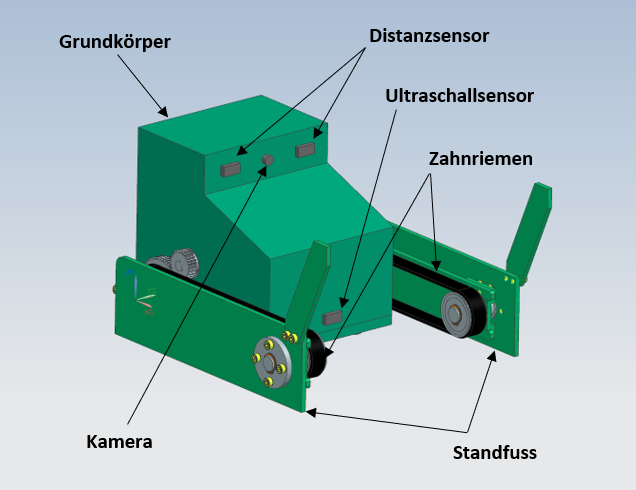
\includegraphics[width=1\textwidth]{img/Treppensteigen/Geraetansicht_final.PNG}
  \centering
  \caption{Konzeptvisualisierung, Ansicht 1}
  \label{fig:konzeptvisualisierung-ansicht1}
\end{figure}

\begin{figure}[H]
  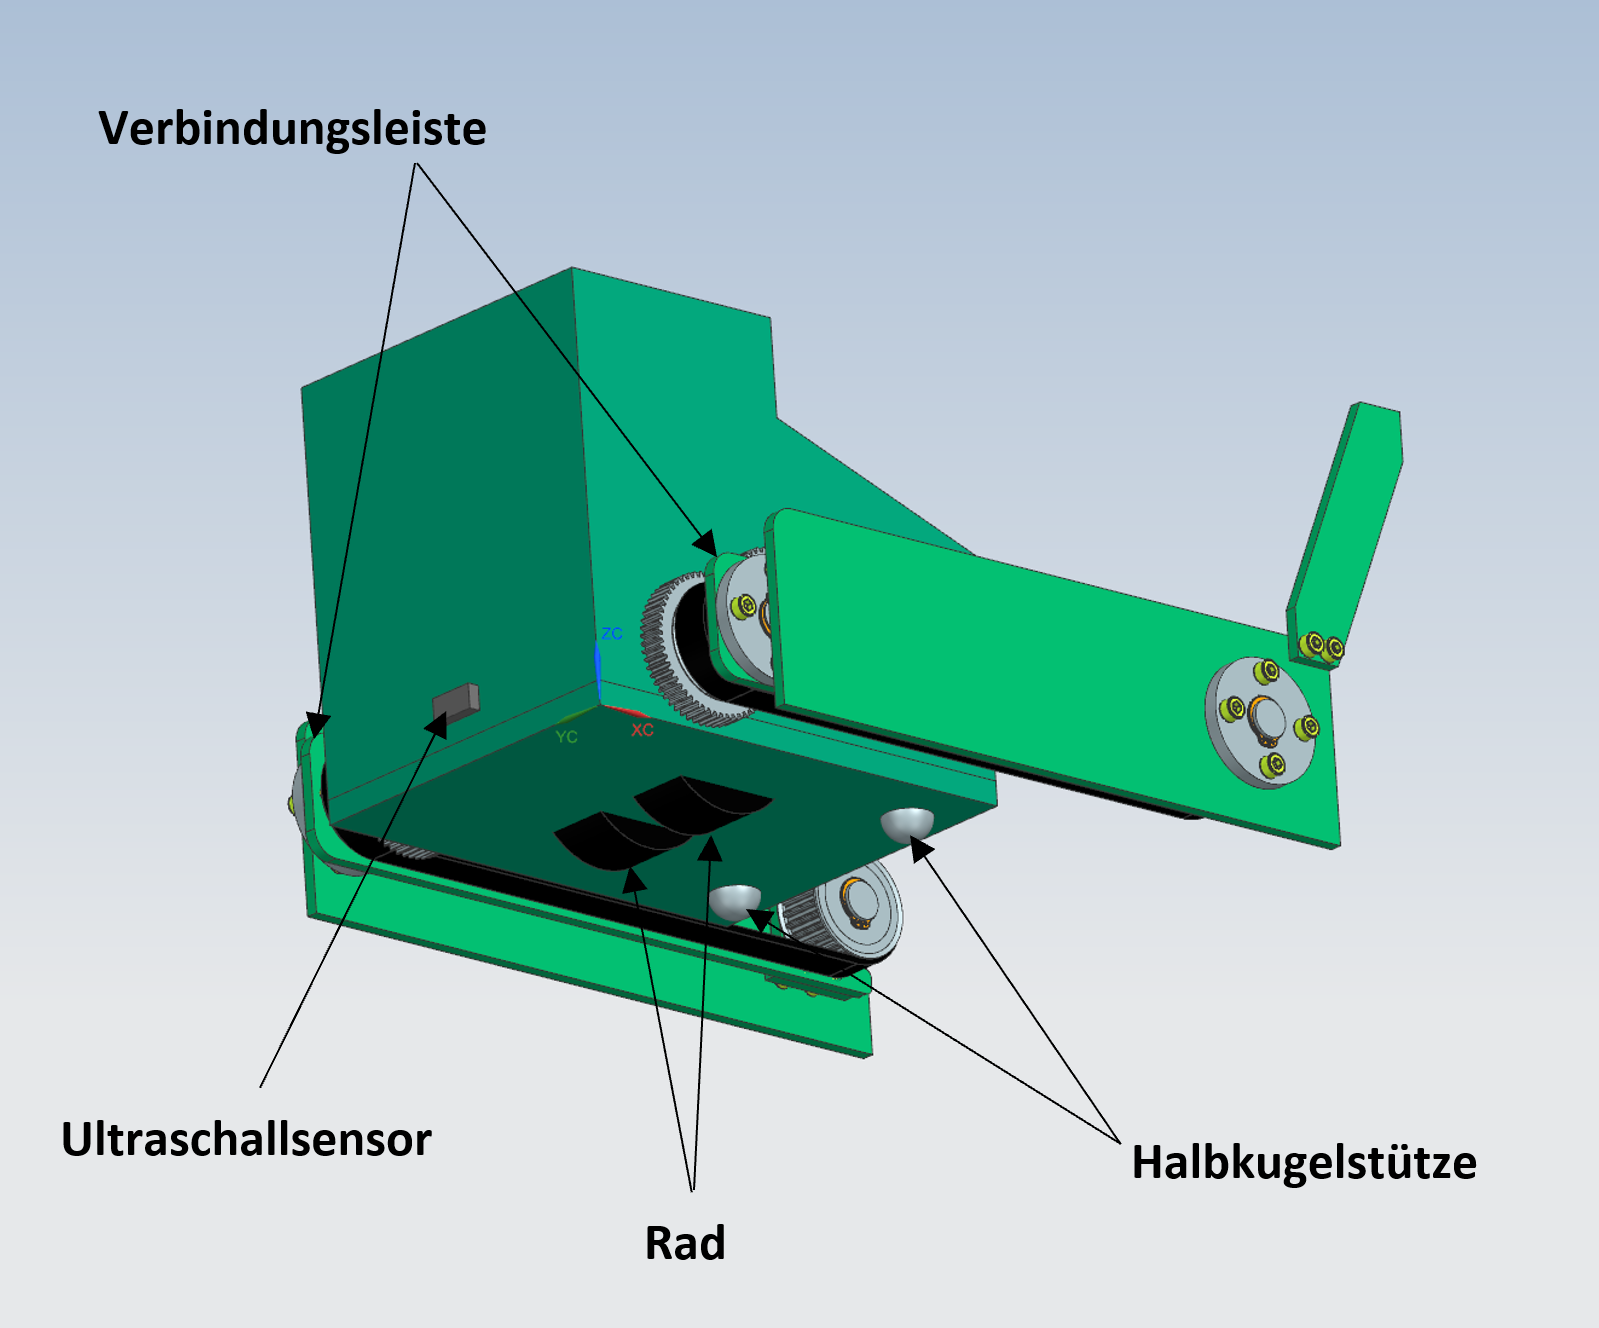
\includegraphics[width=1\textwidth]{img/Treppensteigen/Geraetansicht2_final.PNG}
  \centering
  \caption{Konzeptvisualisierung, Ansicht 2}
  \label{fig:konzeptvisualisierung-ansicht2}
\end{figure}

\newpage

\subsection{Ablauf}
Dieses Unterkapitel gibt einen Überblick über die Zustände, in welchen sich der Roboter während der Erfüllung der Aufgabenstellung befindet. Die Abbildung \ref{fig:gesamtablaufplan} zeigt dies anhand einer Zustandsmaschine. Der Gesamtablauf kann in vier Hauptzustände unterteilt werden. 
\begin{enumerate}
    \item Piktogrammerkennung
    \item Pfadfindung
    \item Treppensteigen
    \item Piktogrammauswahl
\end{enumerate}

\textbf{Piktogrammerkennung}\\
Nachdem der Roboter im Startfeld platziert und der Startknopf gedrückt wurde, beginnt dieser das Piktogramm gemäss \ref{sec:piktogramm-finden-im-startfeld} im Startbereich zu suchen. Sobald das Piktogramm gefunden wurde, wird dies, wie unter \ref{piktogrammerkennung} beschrieben, erkannt. Danach wird die erfolgreiche Erkennung des Piktogramms gemäss \ref{sec:kommunikation} dem Publikum mitgeteilt. 

\textbf{Pfadfindung}\\
Nachdem die Auftragsquittierung abgeschlossen ist, sucht der Roboter die Treppe (siehe \ref{sec:treppe-finden-im-startfeld}). Danach wird der optimale Pfad berechnet (siehe \ref{sec:hindernisserkennung}), damit der Roboter nicht in eine Sackgasse gerät. 

\textbf{Treppensteigen}\\
Ist der optimale Pfad bekannt, so begibt sich der Roboter zum Startpunkt der Treppe.  Sobald der Roboter im richtigen Abstand und senkrecht zur Treppe steht (siehe \ref{sec:ausrichtung-zur-treppe}), beginnt dieser die erste Stufe zu erklimmen. Wie die Erklimmung der Treppe funktioniert, ist unter dem Abschnitt \ref{sec:hubbewegung-analyse} beschrieben. Jedes Mal, wenn sich der Roboter auf einer neuen Stufe befindet, prüft dieser, ob er sich noch auf dem Pfad befinden. Wenn ja, wird sofort die nächste Stufe erklommen. Wenn nein, rotiert er nach links oder rechts, verschiebt sich und rotiert wieder zurück. Mithilfe der Kamera wird die Bewegung auf der Treppe kontrolliert (\ref{sec:orientierung-auf-der-treppenstufe}). Nach dem Verschieben wird die nächste Stufe erklommen. Dieser Ablauf wiederholt sich so lange, bis es keine weiteren Stufen mehr zu erklimmen gibt.

\textbf{Piktogrammauswahl}\\
Sobald sich der Roboter auf der Zielplattform befindet, findet er das im Startbereich erkannte Piktogramm unter denen, die im Zielbereich aufgestellt sind. Wenn er das richtige Piktogramm erkannt hat, fährt er vor dieses hin, um dies dem Publikum zu signalisieren.
\begin{figure}[H]
\begin{center}
    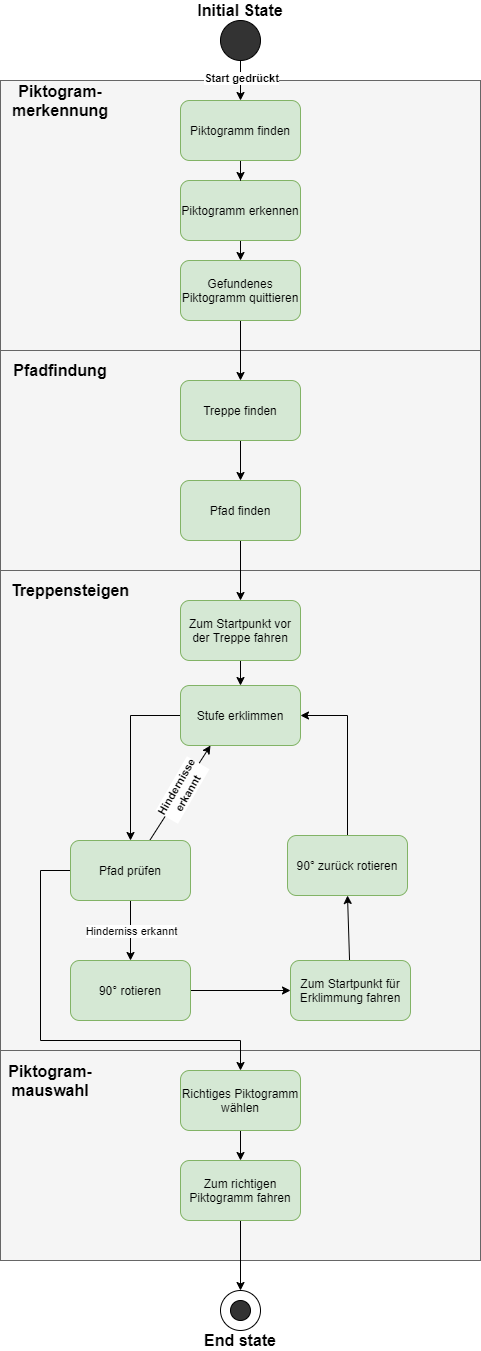
\includegraphics[width=15cm,height=22cm,keepaspectratio]{img/Statemachine.png}
    \caption{Gesamtablauf dargestellt anhand einer Zustandsmaschine}
    \label{fig:gesamtablaufplan}
\end{center}
\end{figure}

\subsection{Treppensteigen}
In diesem Abschnitt wird die Funktion des Treppensteigens genauer erläutert. Dazu gehört eine Beschreibung der einzelnen Komponenten mit den dazugehörenden Berechnungen. Anschliessend werden die Elektromotoren aufgrund der Berechungen definiert. 
\subsubsection{Funktionsprinzip}
Der Grundkörper des Gerätes, in dem Antriebe, Steuerung, Energieversorgung und Orientierungskomponenten enthalten sind, wird auf beiden Seiten mit jeweils einem Standfuss und einer Verbindungsleiste erweitert. Von der Drehachse 1 zur Drehachse 2 wird ein Zahnriemen gespannt (siehe Abbildung \ref{fig:skizze-drehachse-final}). Mit diesen zusätzlichen Elementen soll die Treppe bestiegen werden. Die seitlichen Elemente werden zusammen als Ausleger bezeichnet.

\begin{figure}[H]
  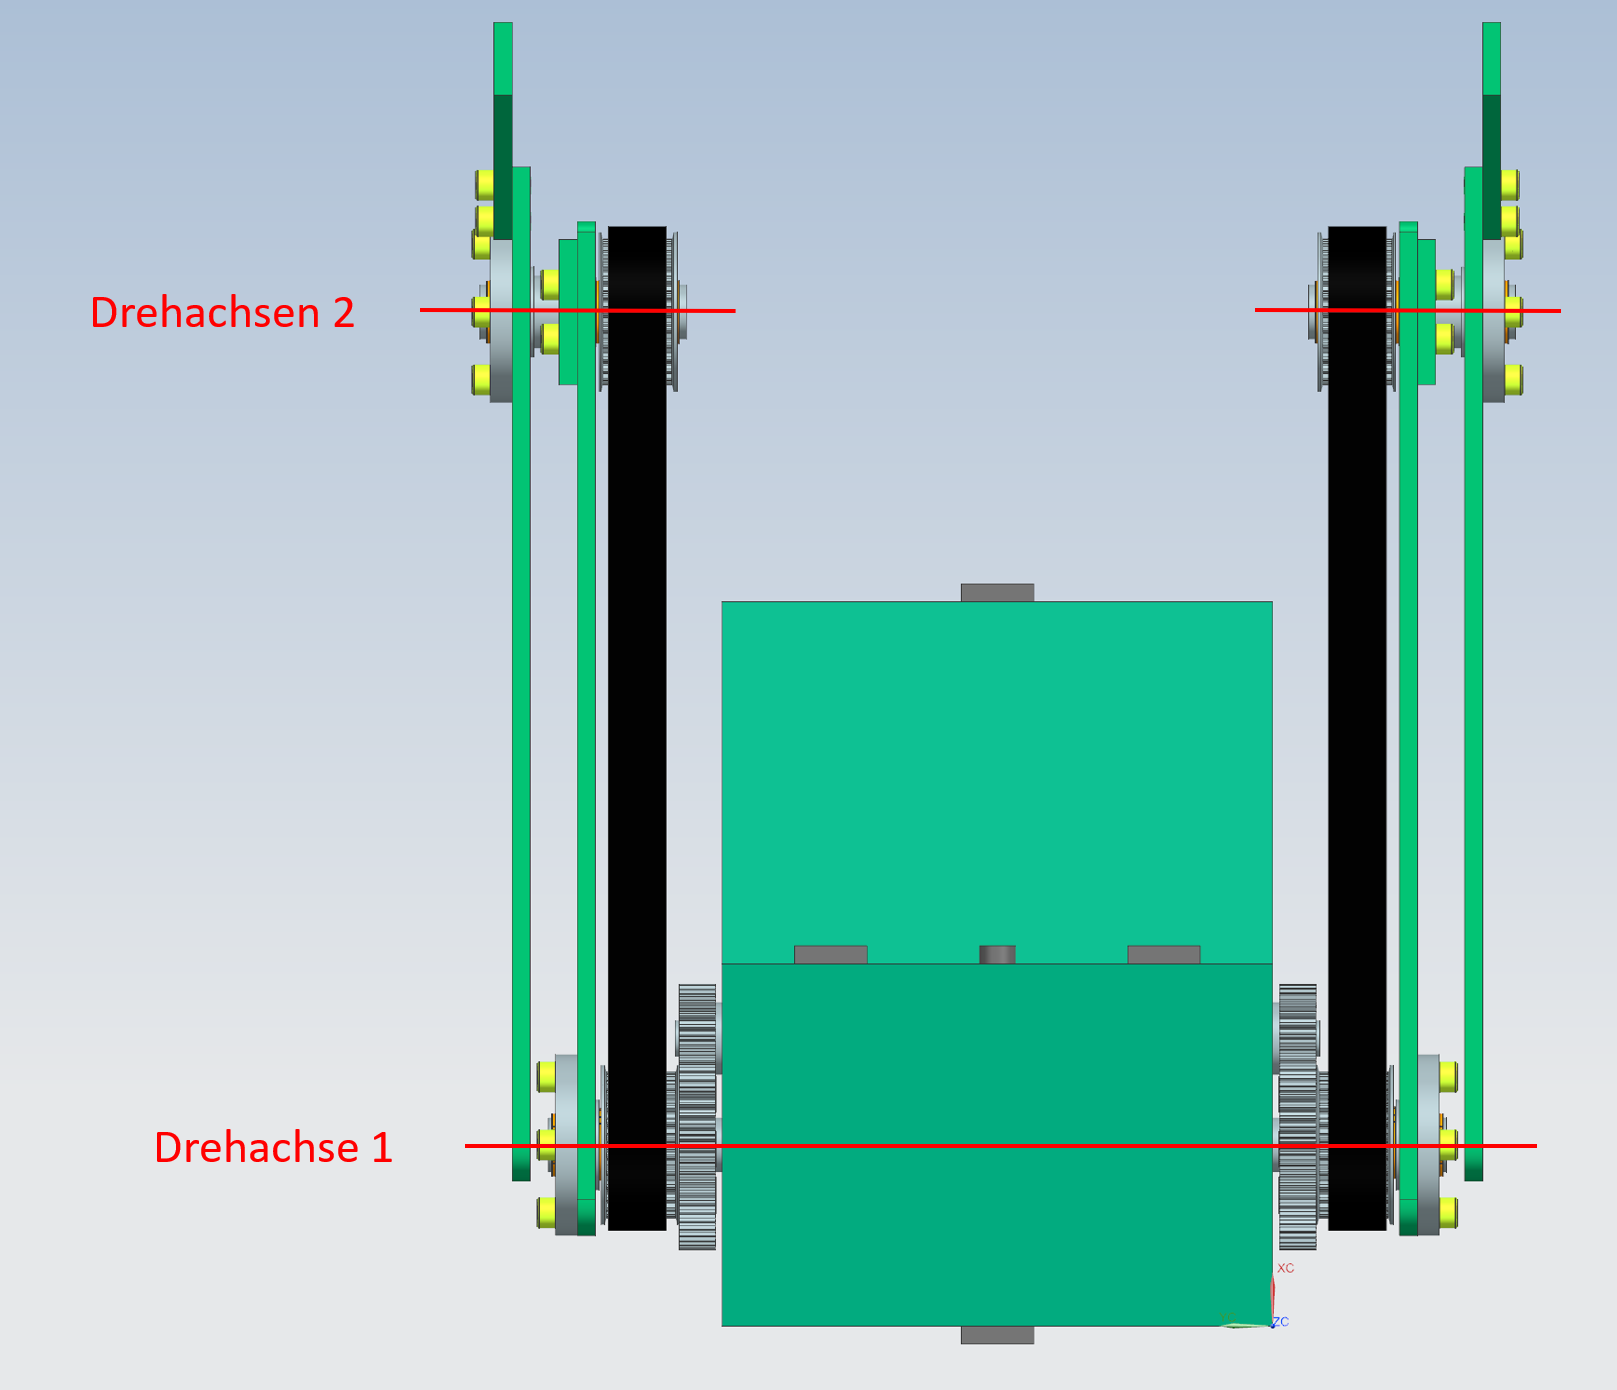
\includegraphics[width=0.8\textwidth]{img/Treppensteigen/Skizze Drehachsen final.PNG}
  \centering
  \caption{Drehachsen}
  \label{fig:skizze-drehachse-final}
\end{figure}

\newpage

Eine Treppenstufe soll mit zwei Hubbewegungen erklommen werden. In einer ersten Hubbewegung bleiben die Standfüsse auf der letzten Stufe und der Grundkörper wird auf die nächste Stufe gehoben. Bei dieser Bewegung wird der Grundkörper horizontal gehalten, wie in Abbildung \ref{fig:1-hubbewegung} ersichtlich.

\begin{figure}[H]
  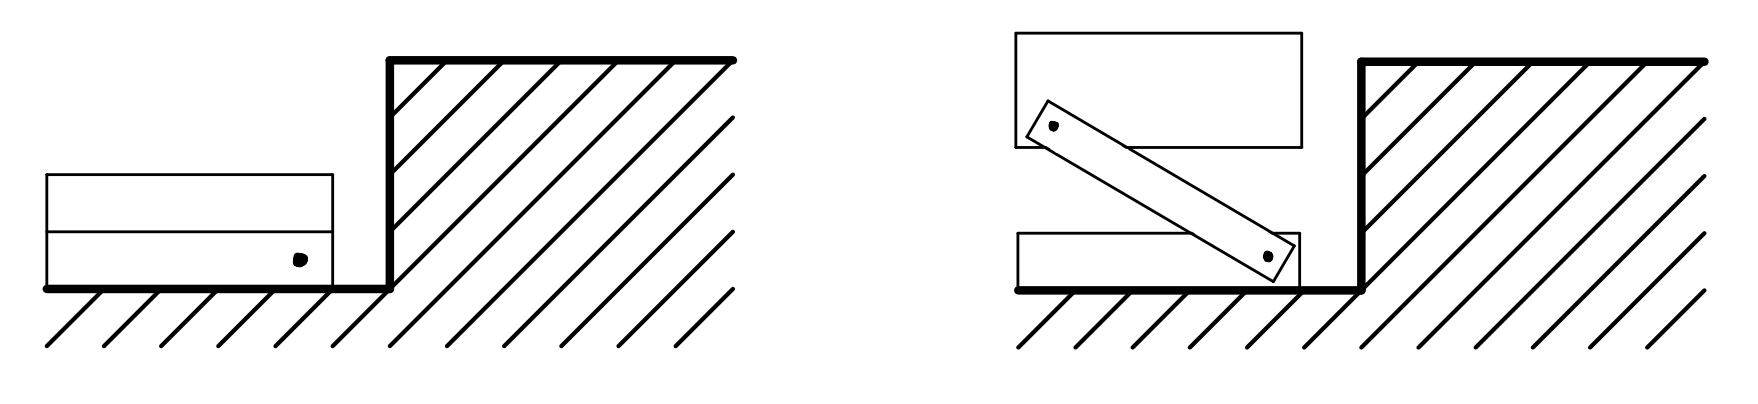
\includegraphics[width=0.9\textwidth]{img/Treppensteigen/1. Hubbewegung Skizze.png}
  \centering
  \caption{Skizze 1. Hubbewegung}
  \label{fig:1-hubbewegung}
\end{figure}
 
Vor der zweiten Hubbewegung soll der Grundkörper komplett über der Trittkante sein. Um das zu erreichen werden die Räder (siehe \ref{sec:fortbewegung}) des Geräts eingesetzt.
 
Bei der zweiten Hubbewegung müssen die Standfüsse auf die nächste Treppenstufe, zurück an die Seiten des Grundkörpers geholt werden, wie in der Abbildung \ref{fig:2-hubbewegung} visuell dargestellt. In der Abbildung \ref{fig:2-hubbewegung} ist oben rechts der kritische Fall zu sehen, wenn die Standfüsse und die Verbindungsleisten in einer Linie sind.

\begin{figure}[H]
  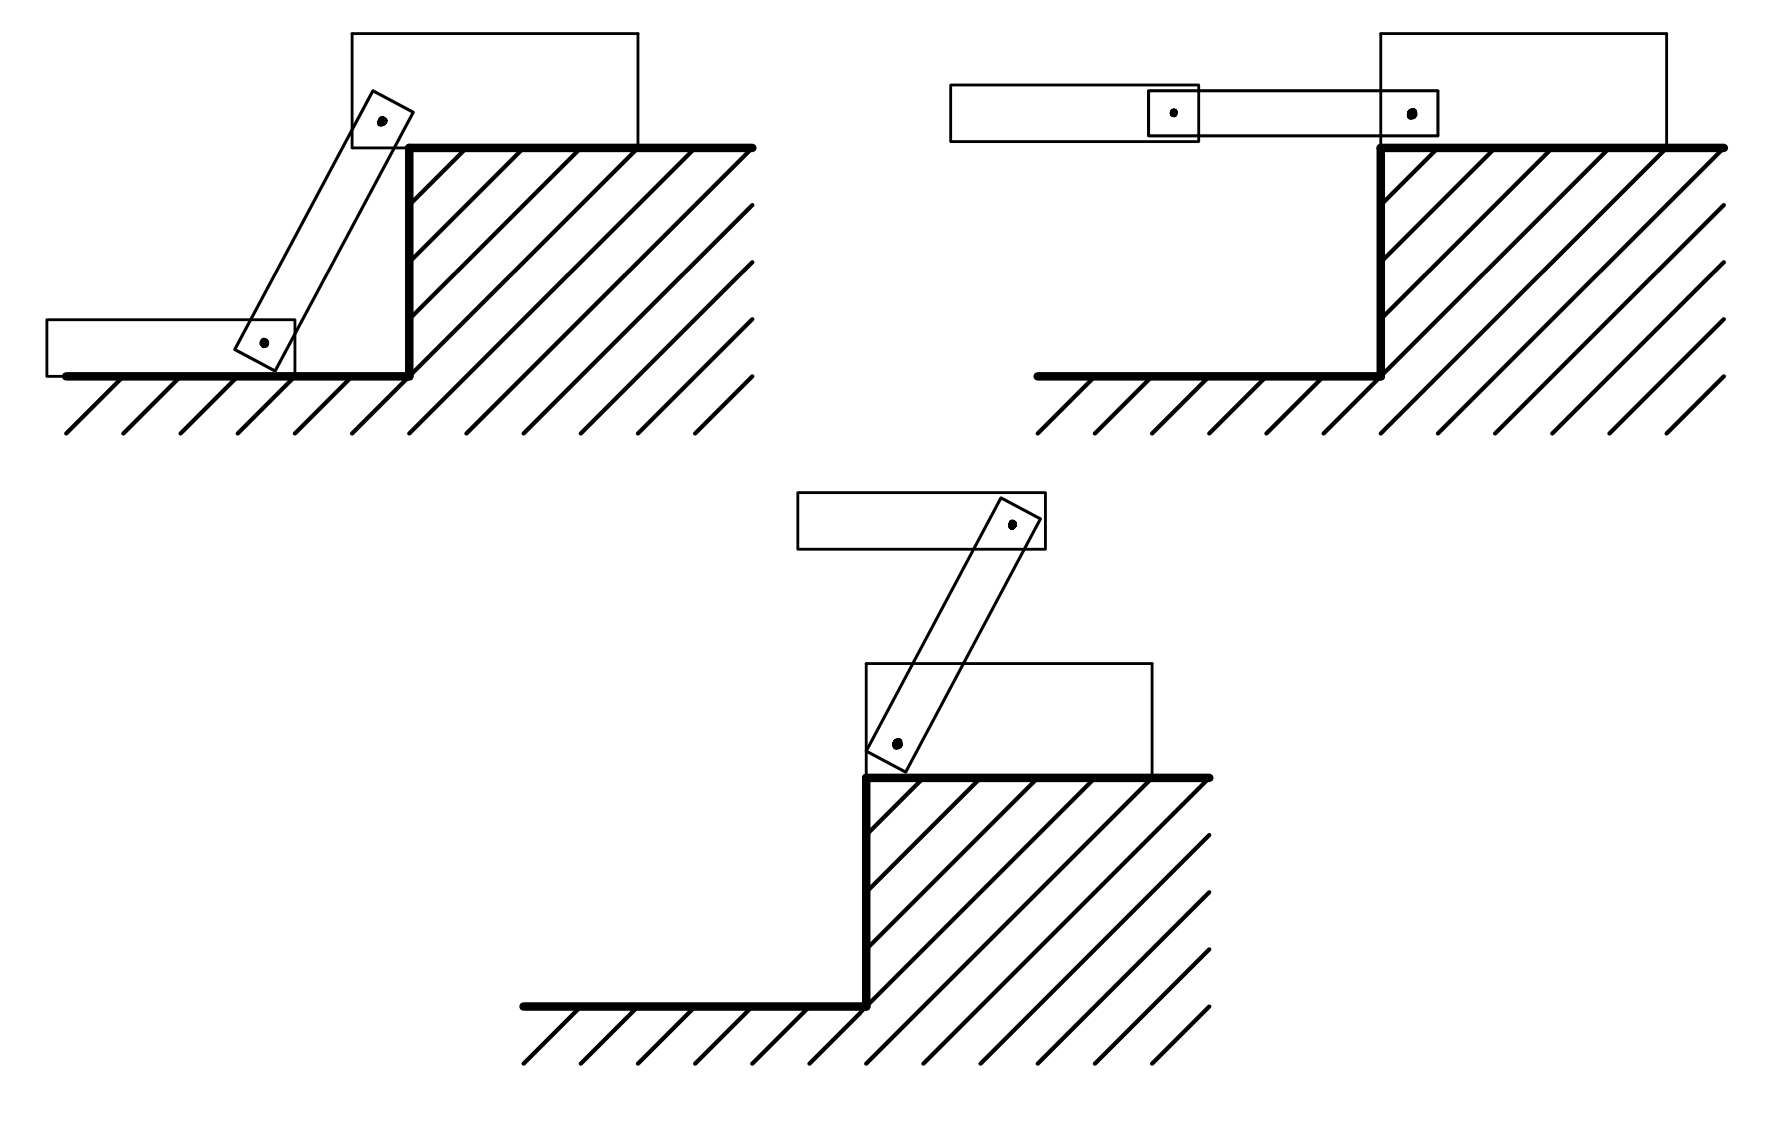
\includegraphics[width=0.9\textwidth]{img/Treppensteigen/2. Hubbewegung Skizze.png}
  \centering
  \caption{Skizze 2. Hubbewegung}
  \label{fig:2-hubbewegung}
\end{figure}

\newpage

\subsubsection{Funktionen der Komponenten}
\textbf{Drehachse 1}\\

Die Verbindungsleisten sind über eine Welle (Welle 1) mit dem Grundkörper verbunden (Drehachse 1). Die Verbindungsleisten sind fest auf der ersten Welle fixiert, sodass sich bei einer Drehung der Welle 1 die Verbindungsleisten um den gleichen Winkel drehen. Das Antriebsrad des Zahnriementriebes ist lose auf der Welle 1 montiert, sodass die Drehbewegungen der Welle und des Antriebsrads des Zahnriemens unabhängig sind.\\

\textbf{Drehachse 2}\\

Die Verbindungsleisten sind mit den Standfüssen bei der zweiten Drehachse verbunden. Die zweite Drehachse ist nicht eine Drehachse, sondern auf beiden Seiten eine einzelne Drehachse. Sie sind aber immer gleich ausgerichtet und werden als eine Drehachse betrachtet (Drehachse 2). Die Standfüsse sind mit den Verbindungsleisten auf beiden Seiten einzeln über kleine, kurze Wellen (Welle 2) verbunden. 

Bei der zweiten Drehachse muss auf beiden Seiten ein Moment aufgebracht werden für die erste Hubbewegung, damit sich die Standfüsse und Verbindungsleisten gegeneinander bei der zweiten Drehachse verdrehen und so der Grundkörper nach oben gehoben wird.

Das Moment bei den zweiten Drehachsen kann nicht direkt mit zwei Einzelnen an die Wellen 2 gekoppelten Motoren aufgebracht werden, da die Motoren bei den Hubbewegungen im Weg wären. Aus diesem Grund muss das Moment für die erste Hubbewegung von der ersten Welle auf die kleinen, kurzen Wellen beidseitig übertragen werden.\\

Für diese Übertragung des Drehmomentes mit einem grossen Achsenabstand eignen sich Zugmittelgetriebe. Da das Gewicht nicht zu gross werden soll, kommen Ketten nicht in Frage. Da das Drehmoment in einem gewissen Verhältnis (i$_{Zahnriemen}$ = 1) und ohne Schlupf übertragen werden soll, eignet sich ein Zahnriemen am besten. Bei der zweiten Welle sind die Standfüsse mit dem Abtriebsrad des Zahnriementriebes gekoppelt und machen so die gleichen Drehbewegungen. Weiter sind bei der zweiten Drehachse die Standfüsse nicht mit den Verbindungsleisten gekoppelt, da sie sich zueinander verdrehen müssen, um die Hubbewegungen auszuführen.

\newpage

\textbf{Hubbewegungen}\\

\textbf{1. Hubbewegung}\\
Für die erste Hubbewegung wird an den Antriebszahnriemenrädern ein Moment eingeleitet. Die Antriebszahnriemenräder sind je mit einem Zahnrad verbunden. Mit einer Übersetzung soll ein erster Elektrogetriebemotor (Motor 1) über eine zusätzliche Welle (Welle 3) diese Antriebszahnriemenräder antreiben. Die Stützen an den Standfüssen greifen unter den nächsten Treppentritt und verhindern, dass bei der ersten Hubbewegung die Ausleger als Ganzes gedreht werden und somit der Grundkörper angehoben wird. Der Motor 1 und die Stützen am vorderen Ende der Ausleger sind in der Abbildung \ref{fig:motor1-und-stützen} ersichtlich. In dieser Abbildung wurde der Grundkörper entfernt, um den Antriebsstrang sichtbar zumachen. Der Motor 1 ist am Grundkörper montiert.

\begin{figure}[H]
  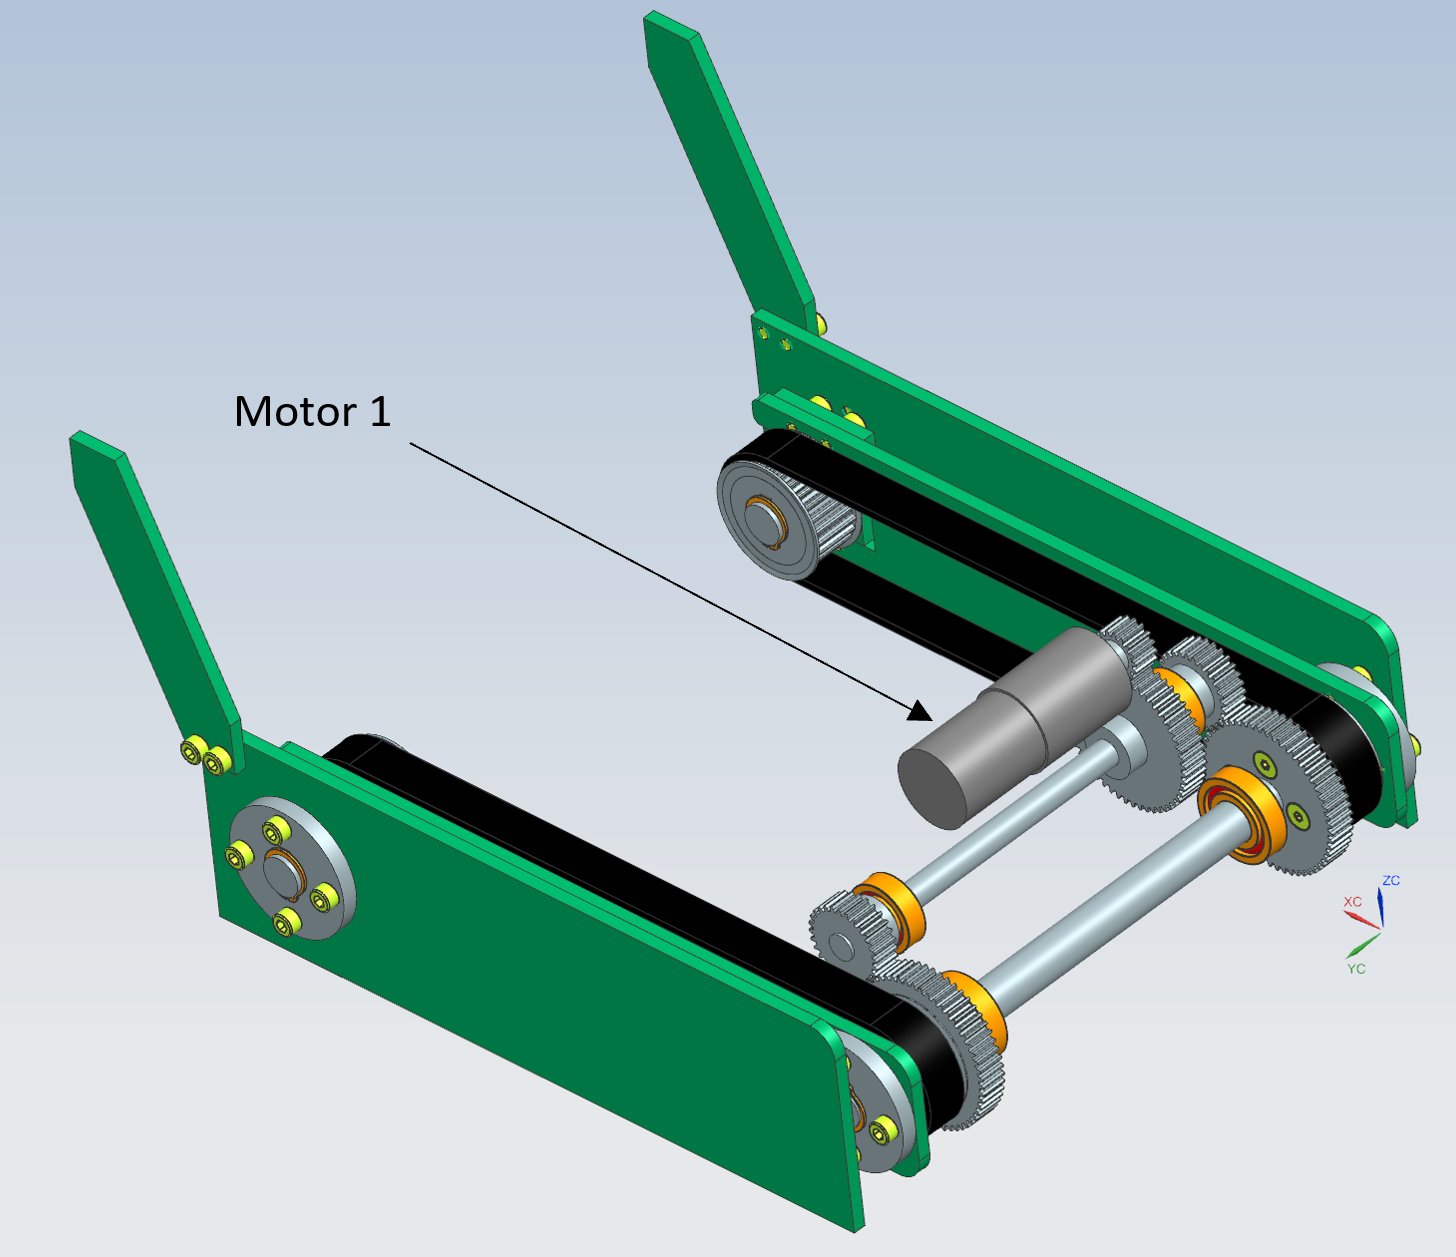
\includegraphics[width=0.7\textwidth]{img/Treppensteigen/Motor 1 final.PNG}
  \centering
  \caption{Kraftübertragung von Motor 1 auf die Antriebsräder der Zahnriemen}
  \label{fig:motor1-und-stützen}
\end{figure}

Notwendiges Moment pro Seite für die 1. Hubbewegung: M$_{erf}$ = 2.7 Nm (siehe Anhang, Berechnungen, Notwendige Momente bei den Hubbewegungen)\\

Übersetzungsverhältnis gesamt: i$_{ges}$ = 6\\

Moment Motor 1: M$_{Motor 1}$ = M$_{erf}$ / i$_{ges}$ = 2.7 Nm / 6 = 0.45 Nm

\newpage

Um den Grundkörper bei der ersten Hubbewegung horizontal halten zu können ist auf der ersten Welle ein Zahnrad angebracht, um mit einem zweiten Elektrogetriebemotor (Motor 2) das Moment der Gewichtskraft des Grundkörpers auszugleichen. Die Kraftübertragung des zweiten Motors ist ist bei der 2. Hubbewegung beschrieben, da das notwendige Moment dort grösser ist.\\

\textbf{2. Hubbewegung}\\
Bei der zweiten Hubbewegung wird die Drehung der Standfüsse bei der zweiten Drehachse mit dem ersten Motor (Motor 1) kontrolliert. Die Drehung der Verbindungsleisten bei der ersten Drehachse wird vom zweiten Motor (Motor 2) angetrieben. Mit diesem Aufbau ist es möglich, die Standfüsse einzeln zu verdrehen. Der Punkt der Kraftübertragung des Motor 2 wird in nachfolgender Abbildung \ref{fig:motor-2} veranschaulicht, wobei der Grundkörper, die Standfüsse und die Zahnriemen ausgeblendet sind. Der Motor 2 ist am Grundkörper angebracht.

\begin{figure}[H]
  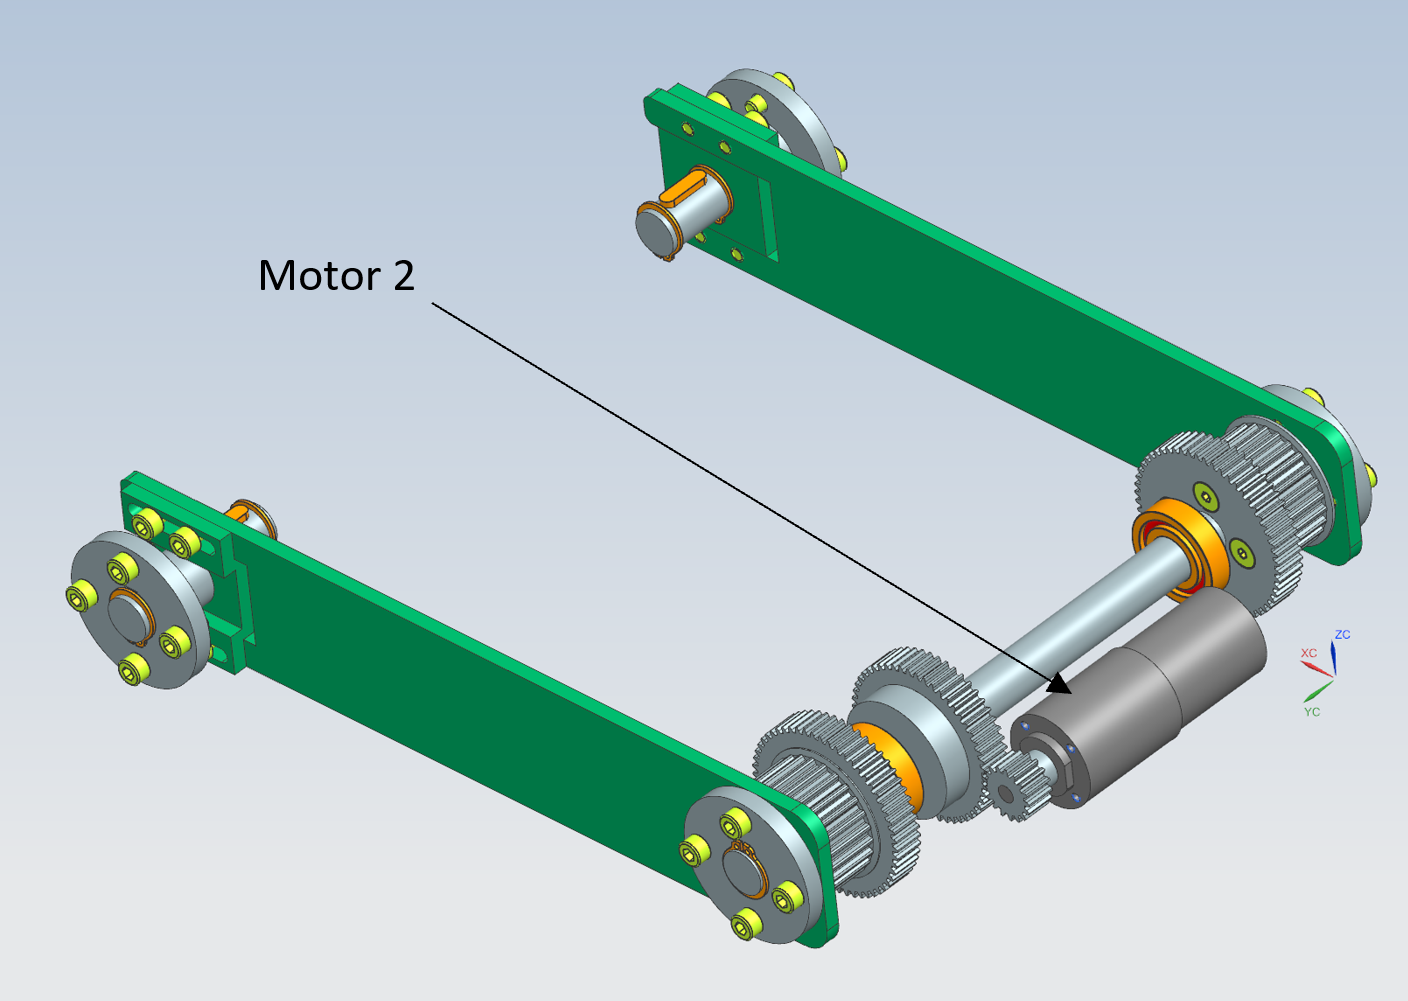
\includegraphics[width=0.8\textwidth]{img/Treppensteigen/Motor 2 final.PNG}
  \centering
  \caption{Aufbau zur Drehung der Ausleger}
  \label{fig:motor-2}
\end{figure}

Notwendiges Moment zur Drehung der Ausleger bei der 2. Hubbewegung (Verbindungsleisten und Standfüsse in einer Linie):

M$_{erf}$ = 3.8 Nm (siehe Anhang, Berechnungen, Notwendige Momente bei den Hubbewegungen)\\

Übersetzungsverhältnis gesamt: i = 3\\

Moment Motor 2: M$_{Motor 2}$ = M$_{erf}$ / i = 3.3 Nm / 3 = 1.1 Nm


\subsubsection{Standsicherheit}
Mit den ersten Abmassen der Komponenten ist eine erste Standsicherheitsbetrachtung bei den zwei Hubbewegungen gemacht worden. Die Skizze in der Abbildung \ref{fig:standsicherheit-1-hubbewegung} zeigt die wirkenden Kräfte bei der ersten Hubbewegung. Dafür wurden die Massen und die Schwerpunkte der Komponenten verwendet (siehe Anhang, Berechnung Massen und Schwerpunkte).\\

\textbf{1.Hubbewegung:}\\

m$_{ges}$ = 4.3 kg

m$_{Grundkoerper}$ = 2.9 kg

m$_{Standfuesse}$ = 1.02 kg

m$_{Verbindungsleisten}$ = 0.38 kg\\

\begin{figure}[H]
  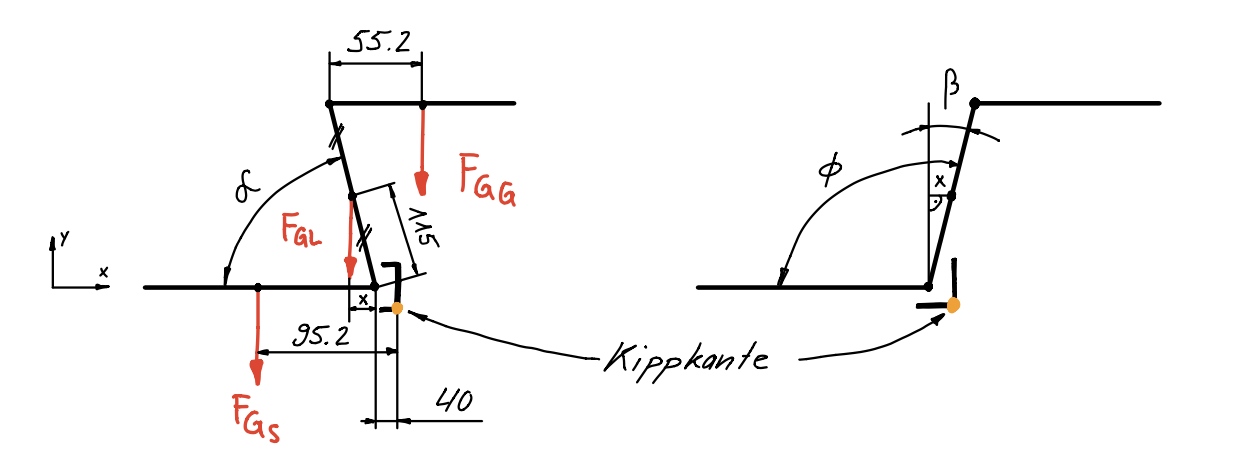
\includegraphics[width=1\textwidth]{img/Treppensteigen/Standsicherheit 1.Hub.png}
  \centering
  \caption{Skizze Standsicherheit bei der 1. Hubbewegung}
  \label{fig:standsicherheit-1-hubbewegung}
\end{figure}

Standsicherheit ist bis \({\alpha} = 90^\circ\) gegeben.

Für \({\alpha} = 90^\circ\) gilt:


\begin{align*}
    M_{Stand} &= F_{GS} * 95.2\ mm + F_{GL} * 40\ mm \\
    &= g\ (m_{Standfuesse} * 95.2\ mm + m_{Verbindungsleisten} * 40\ mm) \\
    &= 9.81\ m/s^2\ * (1.02\ kg * 95.2\ mm + 0.38\ kg * 40\ mm) \\
    &= \underline{\underline{1.09\ Nm}}
\end{align*}

\begin{align*}
    M_{Kipp} &= F_{GG} * 15.2\ mm \\
    &= g\ (m_{Grundkoerper} * 15.2\ mm) \\
    &= 9.81\ m/s^2\ * (2.9\ kg * 15.2\ mm) \\
    &= \underline{\underline{0.43\ Nm}}
\end{align*}

Daraus folgt:
\[M_{Stand} > M_{Kipp}\]

Für \({\alpha} > 90^\circ\) gilt:

\begin{align*}
    F_{GS} * 95.2\ + F_{GL} * (40\ - x) &= (55.2\ + 2x\ - 40)\ ,\text{wenn}\ x < 40 \\
    m_{S} * g * 95.2 + m_{V} * g * (40 - x) &= m_{G} * g * (15.2 + 2x) \\
    m_{S} * 95.2 + m_{V} * 40 - m_{V} * x &= m_{G} * 15.2 + m_{G} * 2x \\
    (2 * m_{G} + m_{V}) x &= m_{S} * 95.2 + m_{V} * 40 - m_{G} * 15.2 \\
    x &= (m_{S} * 95.2 + m_{V} * 40 - m_{G} * 15.2)\ /\ (2 * m_{G} + m_{V}) \\
    x &= 11.6\ mm\ (\text{erfüllt}\ x < 40 mm)
\end{align*}


\({\beta} = \arcsin{(11.6\ mm\ /\ 115\ mm)} = 5.8^{\circ} \)

\({\phi} = 90^{\circ} + {\beta} = 90^{\circ} + 5.8^{\circ} = 95.8^{\circ} \)\\

Bei der ersten Hubbewegung ist die Standsicherheit bis \({\phi} = 95.8^\circ\) gegeben.
\\


\textbf{2.Hubbewegung:}
\begin{figure}[H]
  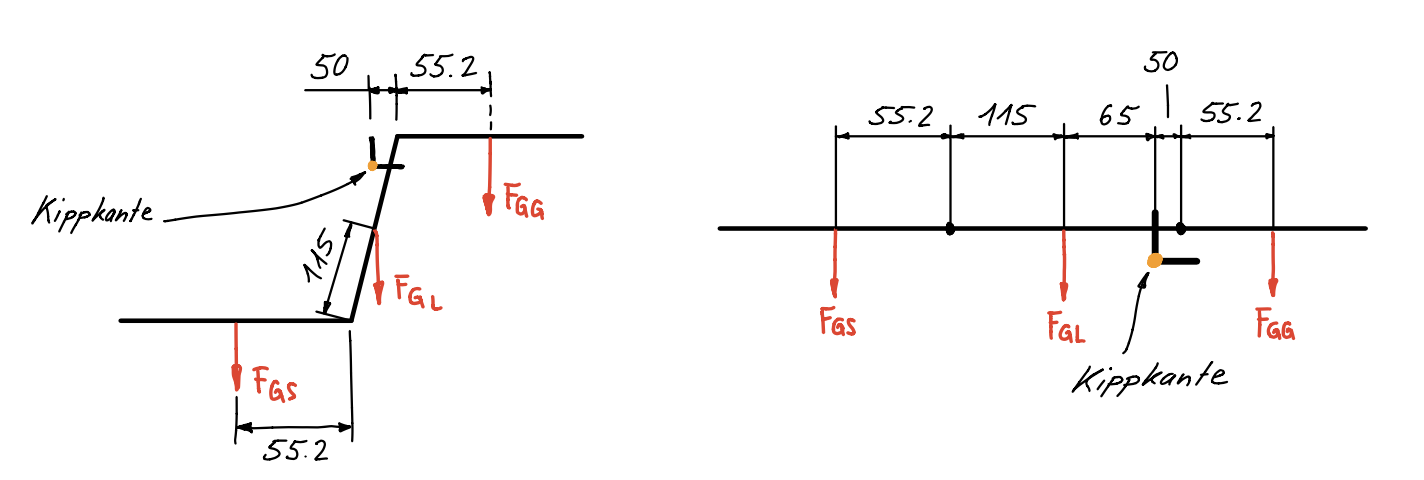
\includegraphics[width=1\textwidth]{img/Treppensteigen/Standsicherheit 2.Hub.png}
  \centering
  \caption{Skizze Standsicherheit bei der 2. Hubbewegung}
  \label{fig:standsicherheit-2-hubbewegung}
\end{figure}

Die Abbildung \ref{fig:standsicherheit-2-hubbewegung} zeigt die Skizze zu den nachfolgenden Berechnungen. Wenn die Standfüsse bei der 2. Hubbewegung waagrecht gehalten werden, ist die kritische Stelle der Hubbewegung, wenn die Standfüsse und die Verbindungsleisten in einer Linie mit dem Drehpunkt des Grundkörpers sind.

In diesem Fall gilt:

\begin{align*}
    M_{Stand} &= F_{GG} * 105.2\ mm \\
    &= g * m_{Grundkoerper} * 105.2\ mm \\
    &= 9.81\ m/s^2\ * 2.9\ kg * 105.2\ mm \\
    &= \underline{\underline{2992.8\ Nmm}}
\end{align*}

\begin{align*}
    M_{Kipp}  &= F_{GS} * (230\ mm + 55.2\ mm - 50\ mm) + F_{GL} * (115\ mm - 50\ mm) \\
    &= g * (m_{Standfuesse} * 235.2\ mm + m_{Verbindungsleisten} * 65\ mm) \\
    &= 9.81\ m/s^2\ (1.02\ kg * 235.2\ mm + 0.38\ kg * 65\ mm) \\
    &= \underline{\underline{2595.7\ Nmm}}
\end{align*}
  
Daraus folgt:
\[M_{Stand} > M_{Kipp}\]

\subsubsection{1. Hubbewegung Analyse}
\label{sec:hubbewegung-analyse}
Mit den ersten Abmassen der Komponenten und der ersten Platziervorstellung auf dem aktuellen Treppentritt wurde analysiert, ob der Grundkörper bei der ersten Hubbewegung mit der Kante des nächsten Treppentrittes kollidiert oder nicht. Es wurde auch berechnet, auf welcher Höhe über dem nächsten Treppentritt und wie weit über der Kante des nächsten Trittes sich der Grundkörper beim kritischen Kippwinkel befindet. Bei dieser Analyse ist der Grundkörper zur Vereinfachung als Quader dargestellt. In der Abbildung \ref{fig:platzierung-auf-treppenstufe-hubbewegung-1} ist die Platzierung mit einem Abstand zur nächsten Stufe von 20 mm ersichtlich.

\begin{figure}[H]
  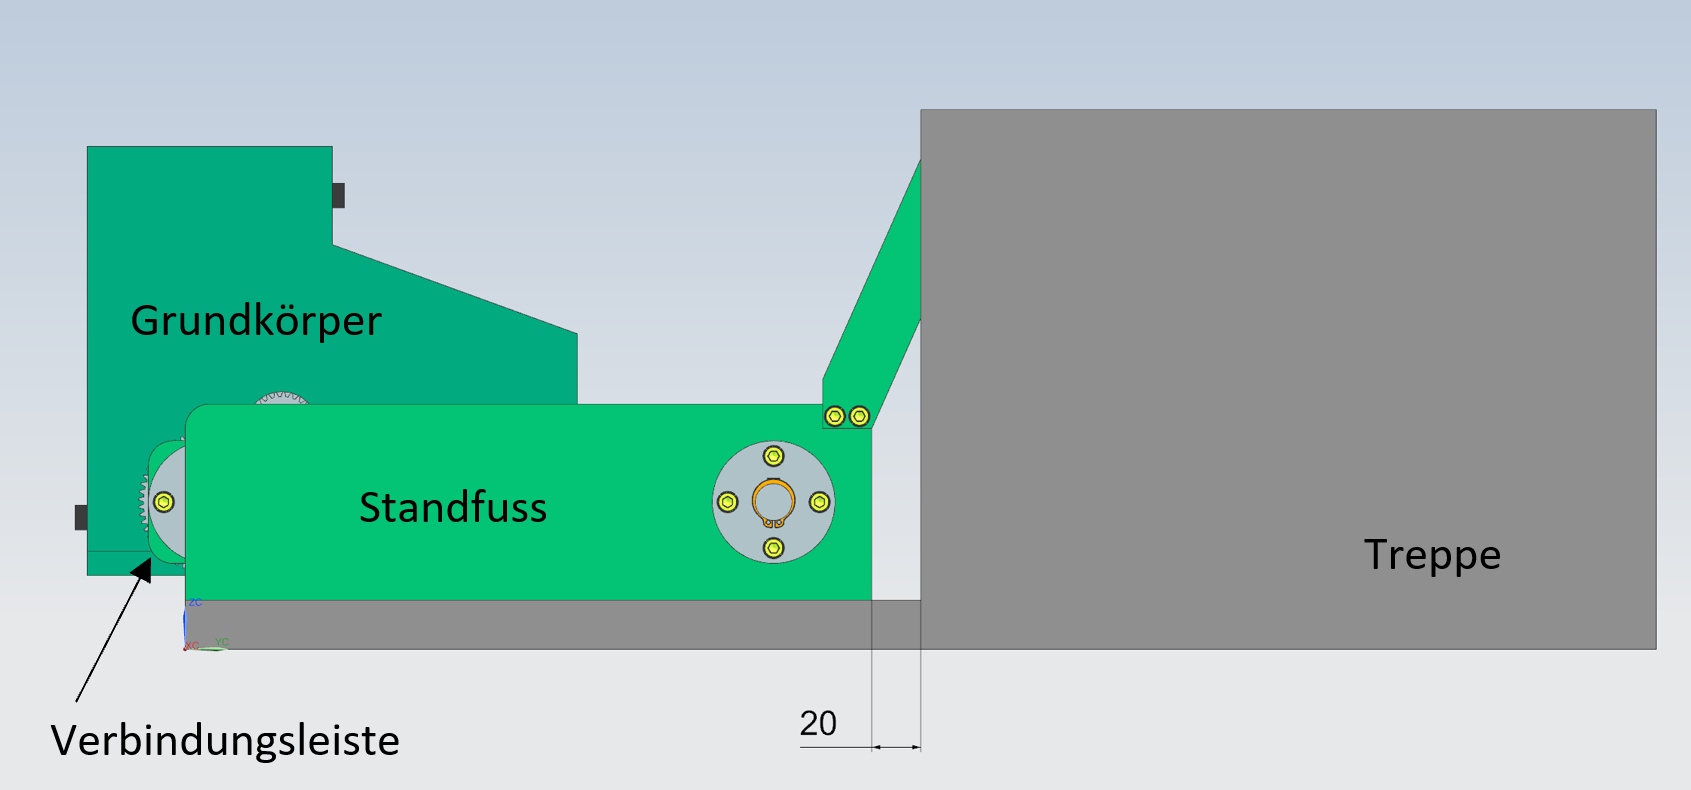
\includegraphics[width=1\textwidth]{img/Treppensteigen/Platzierung auf Treppe final.PNG}
  \centering
  \caption{Platzierung auf aktueller Treppenstufe vor 1. Hubbewegung}
  \label{fig:platzierung-auf-treppenstufe-hubbewegung-1}
\end{figure}

\textbf{Keine Kollision mit Trittkante}\\
Mit dem CAD-Modell wird überprüft, ob der Grundkörper bei der ersten Hubbewegung mit der nächsten Trittkante kollidiert oder nicht. Mit der Platzierungsvorstellung auf dem aktuellen Treppentritt ist eine Bewegung ohne Zusammenstoss möglich.\\
\\

\textbf{Kritischer Kippwinkel erreicht}\\


\begin{figure}[H]
  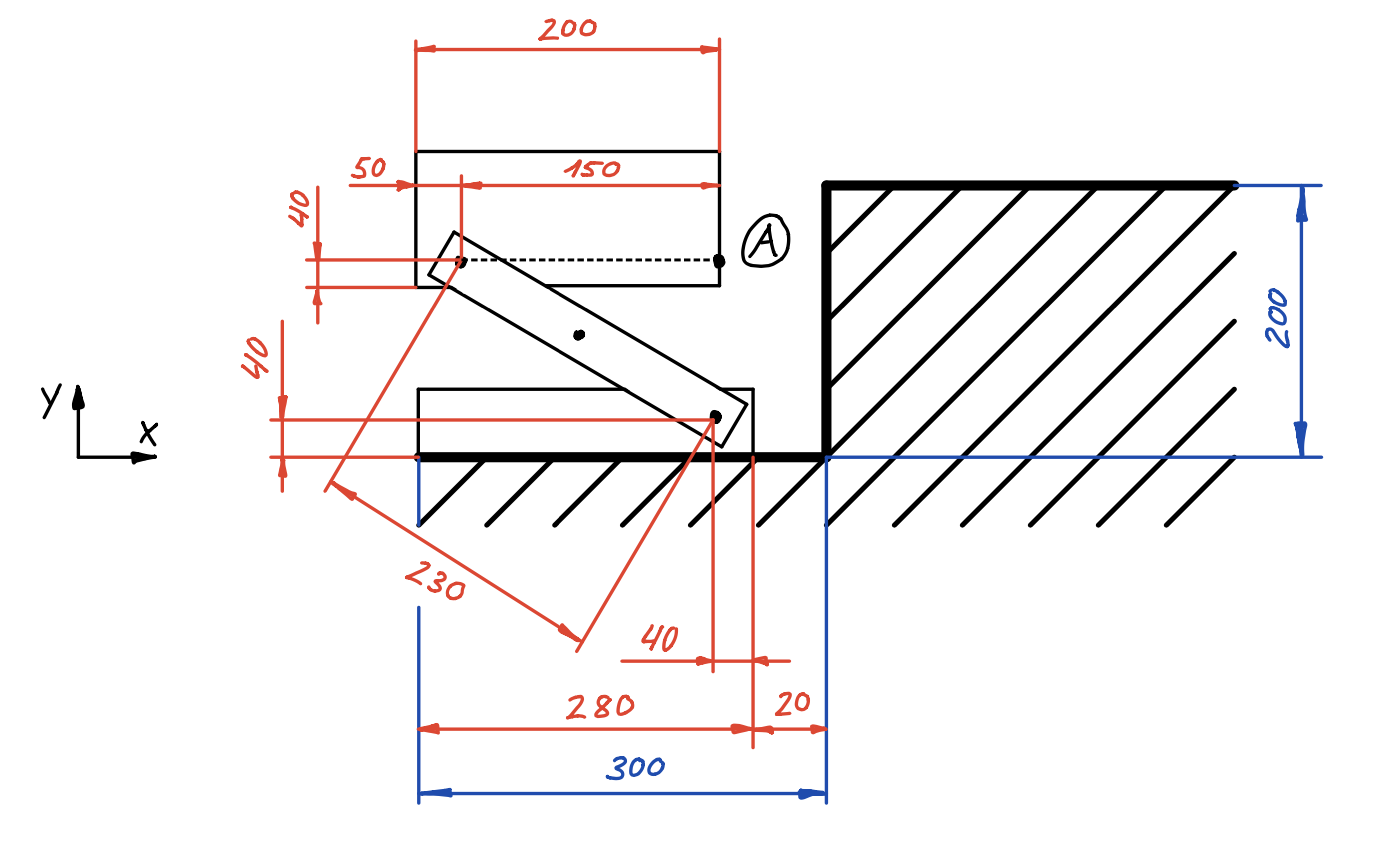
\includegraphics[width=0.7
  \textwidth]{img/Treppensteigen/Skizze Platzierung}
  \centering
  \caption{Skizze Platzierung mit Abmassungen}
  \label{fig:skizze-platzierung}
\end{figure}

\begin{figure}[H]
  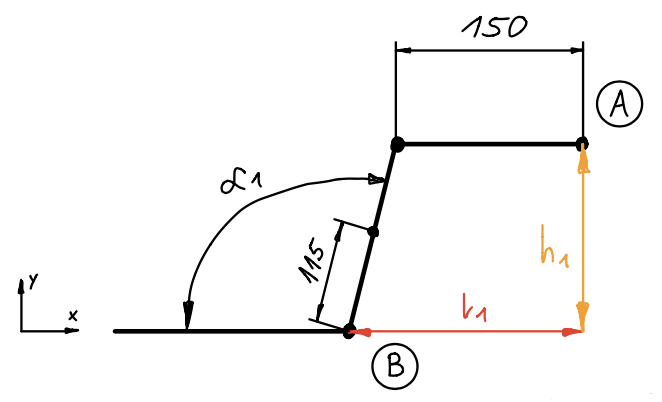
\includegraphics[width=0.6
  \textwidth]{img/Treppensteigen/Analyse 1.png}
  \centering
  \caption{Skizze kritischer Kippwinkel erreicht}
  \label{fig:kritischer-kippwinkel}
\end{figure}

Der in Abbildung \ref{fig:skizze-platzierung} betrachtete Punkt A befindet sich horizontal auf der gleichen Höhe wie der obere Drehpunkt. Im Ausgangszustand ist Punkt A 140 mm in X-Richtung vom nächsten Tritt entfernt. Der Drehpunkt B ist in X-Richtung 60 mm vom nächsten Tritt entfernt.

Wo befindet sich Punkt A, wenn der kritische Kippwinkel \(\alpha_{1} = 95.8^\circ\) erreicht ist?


\(l_{1} = 150 mm + 230 mm * sin(\alpha_{1} - 90^\circ) = 173.2 mm\)

Punkt A in X-Richtung über nächster Trittkante = 173.2 mm - 60 mm = 113.2 mm

Somit ist auch die Kante des Grundkörpers 113.2 mm in X-Richtung über nächster Trittkante.
Die Räder, die sich in der Mitte des Grundkörpers befinden sind also über der nächsten Trittkante.\\

\(h_{1} = 230 mm * cos(\alpha_{1} - 90^\circ) = 228.8 mm\)

Somit sind die Räder in Y-Richtung 28.8 mm über der nächsten Trittkante beim kritischen Kippwinkel, welcher in Abbildung \ref{fig:kritischer-kippwinkel} veranschaulicht wird.\\


\newpage
\subsubsection{Auslegung Elektromotoren}
Der erste Motor benötigt gemäss Berechnungen, ohne Übersetzung und Aufteilung auf zwei Seiten  ein maximales Drehmoment von 5.4 Nm. Dazu passt der Getriebemotor Modelcraft IG320516-41C01 von conrad \cite{Getriebemotor1}. Dieser liefert ein maximales Drehmoment von 7.9 Nm. 
Der zweite Motor benötigt gemäss Berechnungen, ohne Übersetzung ein maximales Drehmoment von 3.3 Nm. Dazu passt der Getriebemotor Modelcraft RB350600-0A101R ebenfalls von conrad \cite{Getriebemotor2}. Dieser liefert ein maximales Drehmoment von 6.1 Nm.

\subsubsection{Sensorik für die Bewegungen}
Die Bewegungen werden durch Elektrogetriebemotoren umgesetzt. Damit die Steuerung die Bewegungen autonom ausführen kann, benötigt die Steuerung Rückmeldungen, in welcher Position sich der Grundkörper und die Standfüsse befinden. Dies soll mittels Tastsensoren realisiert werden.

\begin{figure}[h]
  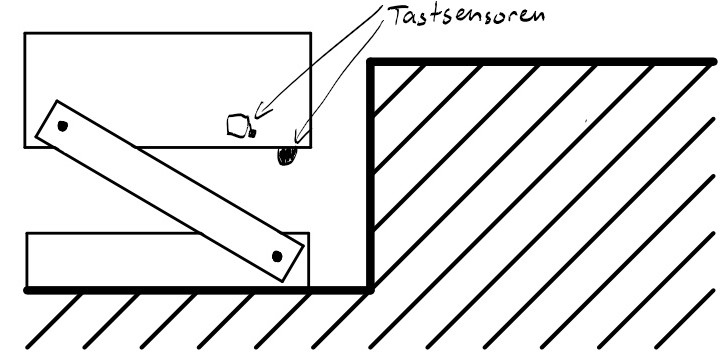
\includegraphics[width=0.6\textwidth]{img/Treppensteigen/Sensoren_Treppensteigen2.png}
  \centering
  \caption{Platzierung der Tastsensoren für die Bewegungen}
  \label{fig:sensoren-treppensteigen2}
\end{figure}

Die Abbildung \ref{fig:sensoren-treppensteigen2} zeigt an welchem Ort der Komponenten die Tastsensoren angebracht werden sollen. Der erste Tastsensor befindet sich unterhalb des Grundkörpers und gibt Rückmeldung, ob der Grundkörper den Boden berührt. Der zweite Tastsensor befindet sich seitlich am Grundkörper und gibt Rückmeldung, wenn sich die Verbindungsleisten am Grundkörper befinden. Dieser Tastsensor ist in Form eines Mikro-Switches mit einem Hebel, welcher gedrückt wird, solange sich die Verbindungsleisten am Grundkörper befinden. Wenn sich der Roboter im Ausgangszustand befindet (eingefahren) sind beide Sensoren aktiv. Danach wird die erste Hubbewegung so lange ausgeführt beziehungsweise der Motor angesteuert, bis sich der Grundkörper auf der Treppe befindet und sich der untere Sensor aktiviert. Danach wird der Motor für die zweite  Hubbewegung solange angesteuert, bis sich die Verbindungsleisten wieder am Grundkörper befinden und die seitlichen Sensoren wieder aktiv sind. Messen, dass sich die Standfüsse, wieder am Grundkörper des Roboters befinden kann man nicht. Es ist geplant, die Ansteuerung des Elektromotors so zu justieren, dass die Standfüsse genau richtig eingefahren sind, sobald sich die Verbindungsleisten am Körper befinden.


\newpage
\subsection{Fortbewegung}
\label{sec:fortbewegung}
Die horizontale Fortbewegung wird mit zwei, unabhängigen voneinander angetriebenen Rädern ermöglicht. Wie in Abbildung \ref{fig:skizze-raeder} gezeigt, werden zusätzlich zu diesen zwei Rädern zwei Stützpunkte benötigt, damit der Grundkörper nicht den Boden berührt. Verwendet werden zwei, damit der Roboter bei der Hubbewegung auf die nächste Stufe gerade bleibt. Diese Stützpunkte werden auf einem Tastsensor montiert und sind in der Form einer Halbkugel, um einfaches gleiten zu gewährleisten und sicherzustellen, dass der Stützpunkt auf der Treppe nicht hängen bleibt.

\begin{figure}[H]
  \includegraphics[width=0.8\textwidth]{img/Fortbewegung/Skizze Räder.png}
  \centering
  \caption{Skizze Räder mit Halbkugelstützen}
  \label{fig:skizze-raeder}
\end{figure}

Dieses Fortbewegungsprinzip ermöglicht es dem Gerät, sich an Ort und Stelle zu drehen, indem die Räder in die entgegengesetzt Richtung angesteuert werden. Der Roboter kann sich somit im Start- und Zielbereich in alle Richtungen schnell und flexibel bewegen. Dies ist zu Beginn, um vor die Treppe zu fahren, und beim abschliessenden Suchen des Zielpiktogramms vorteilhaft. Um auf den Treppenstufen nach links oder rechts auszuweichen, soll sich das Gerät zuerst um 90$^\circ$ drehen, dann geradeaus fahren und sich anschliessend wieder um 90$^\circ$ drehen, sodass sich das Gerät an der Position für den nächsten Treppensteigprozess rechtwinklig vor dem nächsten Treppentritt befindet.

\newpage

\subsubsection{Berechnung der Antriebsleistung}
Für eine erste Berechnung der notwendigen Antriebsleistung zur Fortbewegung werden ein Raddurchmesser und eine maximale Wunschgeschwindigkeit angenommen. Die Räder sollen aus Gummi sein. Die Materialien, die der Roboter befahren muss sind Holz im Startbereich und Aluminium auf der Treppe. Für die Berechnung des notwendigen Antriebsmoments auf Holz und Aluminium, ohne durchrutschen der Räder, wird ein Reibungskoeffizent \cite{Reibung} für die Paarung Gummi-Metall verwendet. Wird das gleiche berechnete Moment auf der Holzunterlage aufgebracht, ist das durchrutschen weniger kritisch, da die Reibung zwischen dem Holz und den Gummirädern grösser ist. In der Abbildung \ref{fig:skizze-radberechnung} werden alle wirksamen Kräfte und deren Wirkungsrichtung veranschaulicht.

\begin{figure}[H]
  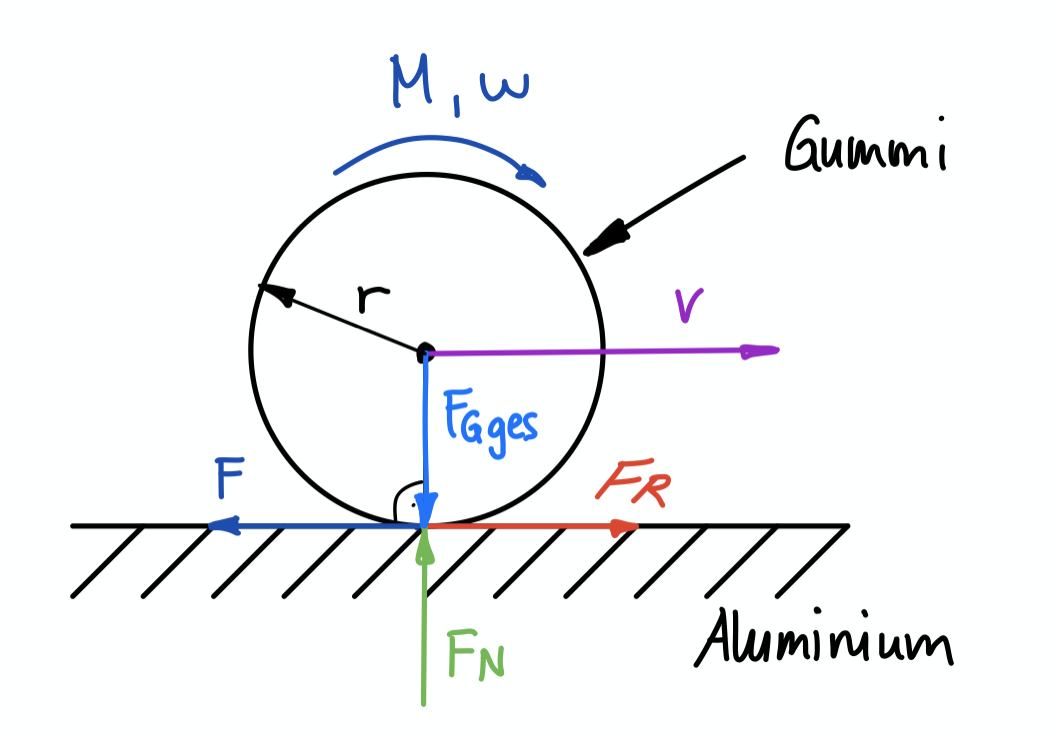
\includegraphics[width=0.8\textwidth]{img/Fortbewegung/Radberechnung.png}
  \centering
  \caption{Skizze zur Radberechnung}
  \label{fig:skizze-radberechnung}
\end{figure}

\newpage

Betrachtet wird ein Rad. Ein Rad trägt näherungsweise 1/2 des Gesamtgewichts.

m$_{ges}$ = 4.3 kg

d$_{Rad}$ = 70 mm

v$_{Wunsch}$ = 1 m/s

\( \mu_{Gummi-Aluminium} = 0.5\)

\[F_{Gges} = m_{ges} * g = 4.3\ kg * 9.81\ m/s^2\ = 42.2\ N \]

\[F_N = F_{Gges}\ /\ 2 = 42.2\ N\ /\ 2 = 21.1\ N \]

\[F = F_R = F_N * {\mu_{Gummi-Aluminium}} = 21.1\ N * 0.5 = 10.55\ N\]

\[M_{max} = F * r = 10.55\ N * 0.035\ m = 0.37\ Nm\]

\[\text{Kein Rutschen}: \omega_{max} = v_{Wunsch}\ /\ r = 1\ m/s\ /\ 0.035\ m = 28.6\ rad/s\]


\subsubsection{Auswahl der Motoren für die Fortbewegung}
Für die Fortbewegung am Boden benötigt der Roboter 2 Motoren. Gemäss Berechnung ist das maximal vorhandene Drehmoment je Motor ein Drehmoment von 0.37 Nm. Zusätzlich sollen die Motoren mit einem Encoder ausgestattet sein, um eine 90\textdegree-Drehung ausführen zu können beziehungsweise um den zurückgelegten Weg ermitteln zu können. Eine Auswahl für diesen Motortyp ist der DC 12 V DIY Encoder Getriebemotor von amazon \cite{MotorEncoder}. Dieser liefert ein maximales Drehmoment von 0.9 Nm. 
Die Funktion eines Encoders oder Inkrementalgeber kann wie folgt beschrieben werden: Ein Inkrementalgeber hat 2 Ausgangssignale \glqq A\grqq{} und \glqq B\grqq{}. Die Abbildung \ref{fig:encoder-signal} zeigt den zeitlichen Verlauf der Kanäle. Ein Signal ist jeweils um 90\textdegree\ versetzt. Durch Drehen des Drehgebers im Uhrzeigersinn, wird der \glqq A\grqq{} Puls um 90\textdegree{} vor dem \glqq B\grqq{} Puls gesendet. Durch Drehen der Welle gegen den Uhrzeigersinn wird der \glqq B\grqq{} Puls vor dem \glqq A\grqq{} Puls gesendet. Dadurch kann per Software die Drehrichtung und die Geschwindigkeit ermittelt werden.

\begin{figure}[H]
  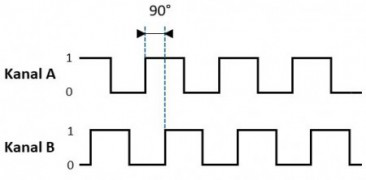
\includegraphics[width=0.5\textwidth]{img/Fortbewegung/Increment Encoder Signal.png}
  \centering
  \caption{Kanal A und B eines Inkrementalgebers}
  \label{fig:encoder-signal}
\end{figure}


\subsubsection{Überwachung der Fortbewegung}
Um sicherzustellen, dass der Roboter nicht von der Treppe fällt oder in ein Hindernis hineinfährt, müssen die Bewegungen überwacht werden.

Um das Herunterfallen abzuwenden, werden unterhalb des Roboters Distanzsensoren angebracht, welche erkennen, wann eine Ecke der Maschine die Treppe verlässt. Dies wird in Abbildung \ref{fig:sensoren-fortbewegung1} gezeigt. Diese Sensoren sind redundant und sind ausschliesslich für den Fall verbaut, dass beim Traversieren auf der Treppe ein Fehler geschieht.
Die Positionierung auf der Treppe wird grösstenteils mit der Kamera überwacht. Zusätzlich wird in Front-, und Rückrichtung je ein Ultraschallsensor eingebaut. Dies wird in erster Linie dafür gemacht, die Kamera zu unterstützen und um ein besseres Bild der Lage zu erhalten. Ausserdem werden Ultraschallsensoren und nicht \acrshort{tof}-Distanzsensoren verwendet, da diese ein breiteres Bild ergeben und auch hochkant stehende Hindernisse erkennen können.
Damit die Distanz zur Treppe für das Treppensteigen richtig eingeschätzt werden kann, werden zwei Sensoren in Frontalrichtung auf Höhe der Treppenkante montiert.

\begin{figure}[h]
  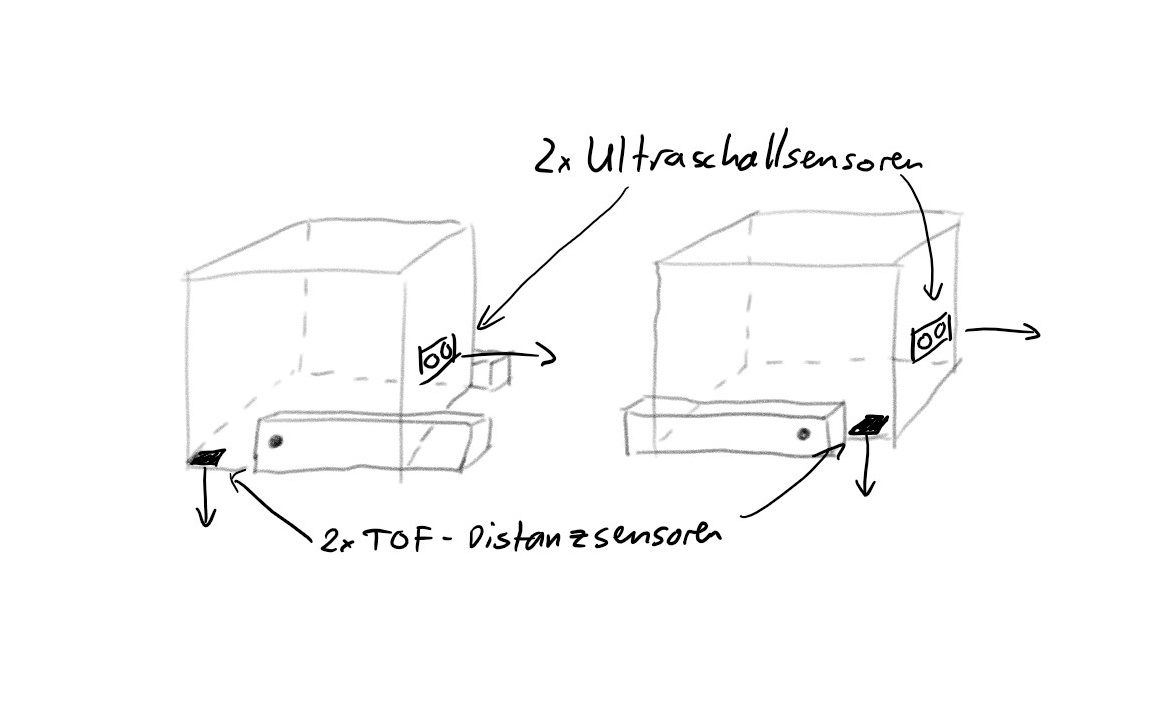
\includegraphics[width=0.65\textwidth]{img/Fortbewegung/Skizze_Sensoren_Fortbewegung_1.png}
  \centering
  \caption{Sensoren für die Fortbewegung}
  \label{fig:sensoren-fortbewegung1}
\end{figure}


\subsection{Elektrosteuerung}
Die Steuerung der Elektrokomponenten wie Motoren, Sensoren und Kameras erledigt ein Raspberry Pi. Das Bord steuert nicht nur die Eingänge, der Sensoren und steuert die Motoren an, sondern es verarbeitet auch die Bilder und berechnet den abzufahrenden Pfad. Das Raspberry Pi ist das Gehirn des Roboters.


\subsubsection{Kapazität Akku}
Die elektrischen Komponenten des Roboters werden mit Energie versorgt. Diese Energie soll ein \acrshort{lipo}-Akku liefern. Um die Kapazität grob bestimmen zu können werden die Verbräuche der Komponenten in der Tabelle \ref{tab:stromverbrauch-der-komponenten} zusammengetragen:   

\begin{table}[H]
\centering
\begin{tabular}{|l|r|}
\hline
\textbf{Komponenten} & \textbf{Leistung (max)} \\ \hline
4x \acrshort{tof}-Abstandssensoren & 0.08 W \\ \hline
2x Ultraschallsensor & 0.15 W \\ \hline
Motor 1+2 Treppensteigen & 4.39 W \\ \hline
Motor 1+2 Fortbewegung & 5.00 W \\ \hline
Raspberry Pi 3 mit Kamera & 3.00 W \\ \hline
4x H-Brücken & 0.20 W \\ \hline
\textbf{Total} & \textbf{12.82 W} \\ \hline
\end{tabular}
\caption{Stromverbrauch der Komponenten}
\label{tab:stromverbrauch-der-komponenten}
\end{table}


Der Roboter muss gemäss Anforderungskatalog 12 min fahren können. Die Energie lässt sich wie folgt berechnen:
\[E = P * t = 12.82\ W * \frac{12\ min}{60} = 2.564\ Wh\]
Daraus lässt sich die Kapazität berechnen:
\[C = \frac{E}{U} = \frac{2.564\ Wh}{12\ V} * 1000 = 214\ mAh\]
Ein dazu passender Akku mit genügend Reserven ist das DroneArt Modellbau-Akkupack (LiPo) 14.8 V 1550 mAh von conrad \cite{Akku}.


\newpage
\subsection{Umgebungserkennung}
\subsubsection{Finden des Piktogramms im Startfeld}
\label{sec:piktogramm-finden-im-startfeld}
Um im Startfeld das Piktogramm zu finden wird die Kamera verwendet. Hier ist geplant, mit einem FindContours-Algorithmus \cite{OpenCV-Fining-Contours} in OpenCV alle Konturen mit vier Eckpunkten herauszufiltern. Dabei werden diese gefundenen Konturen mit vier Eckpunkten nach der Grösse der Fläche sortiert. Dabei wird davon ausgegangen, dass die Grösste dieser Konturen das Schild mit dem Piktogramm ist.\\ 
Sobald eine plausible Kontur gefunden wurde kann das Bild bereits für die Piktogrammerkennung vorbereitet werden. Hierbei wird es auf die \acrfull{roi}, also auf die für die Aufgaben interessanten Stellen begrenzt und optional mit der getGeometricTransform-Methode von OpenCV eine Top-Down-View auf das Bild erstellt. Da es sich bei den Piktogrammen um Schwarz-Weiss-Bilder handelt, kann man hier noch leicht die unterschiedlichen Lichtverhältnisse herausfiltern, in dem man noch eine Threshold anwendet, somit werden die aufgenommenen Farben ausschliesslich auf Schwarz und Weiss begrenzt, was in erster Linie die Weiterverarbeitung vereinfacht.
Folgend eine Auflistung der geplanten Bildverarbeitungsschritte:
\begin{enumerate}
    \item Verkleinerung
    \item In Graustufen konvertieren 
    \item Verzerren
    \item Erkennen von Kanten (Canny edge detection)
    \item Finden der Konturen
    \item Sortieren aller Rechteckigen Konturen nach Fläche
    \item Einzeichnen der Konturen mit grösster Fläche auf dem Originalbild
    \item Auf \acrshort{roi} zuschneiden
    \item Optional: Top-Down-View auf das Bild erstellen (getGeometricTransform())
    \item Thresholding
\end{enumerate}

\subsubsection{Finden der Treppe im Startfeld}
\label{sec:treppe-finden-im-startfeld}
Für das Finden der Treppe soll der gleiche Algorithmus verwendet werden, mit welchem auch das Path-Finding realisiert werden soll. Sobald also das Piktogramm gefunden und der Auftrag quittiert wurde, macht sich der Roboter auf die Suche nach der Treppe. Danach fährt der Roboter an den Start des definierten Pfades. Damit die Ausrichtung zur Treppe genau 90$^\circ$ beträgt, ist der Roboter mit zwei Distanzsensoren an der Vorderseite ausgestattet. Die beiden gemessenen Distanzen zur ersten Treppenstufe können so gleich gehalten werden.

\subsubsection{Ausrichtung zur Treppe}
\label{sec:ausrichtung-zur-treppe}
Im Abschnitt Zusätzliche Evaluation - Ausrichtung zur Treppenstufe, welcher sich im Anhang befindet, wurden Tastsensoren, Kraftsensoren, Distanzsensoren und Kameras einander gegenübergestellt und verglichen. Das Ergebnis der Evaluation sind Distanzsensoren, da diese simpel, genau und günstig sind und man nicht ganz an die Treppe heranfahren muss.\\
Um die Ausrichtung zur Treppe zu bestimmen, werden also zwei Distanzsensoren verwendet, welche auf Treppenstufenhöhe an der Vorderseite des Roboters angemacht werden. In Abbildung \ref{fig:distanzsensoren} wird dies veranschaulicht. Der Roboter ist senkrecht ausgerichtet, wenn beide Distanzsensoren den gleichen, definierten Abstand zur Treppenstufe erkennen.

\begin{figure}[h]
  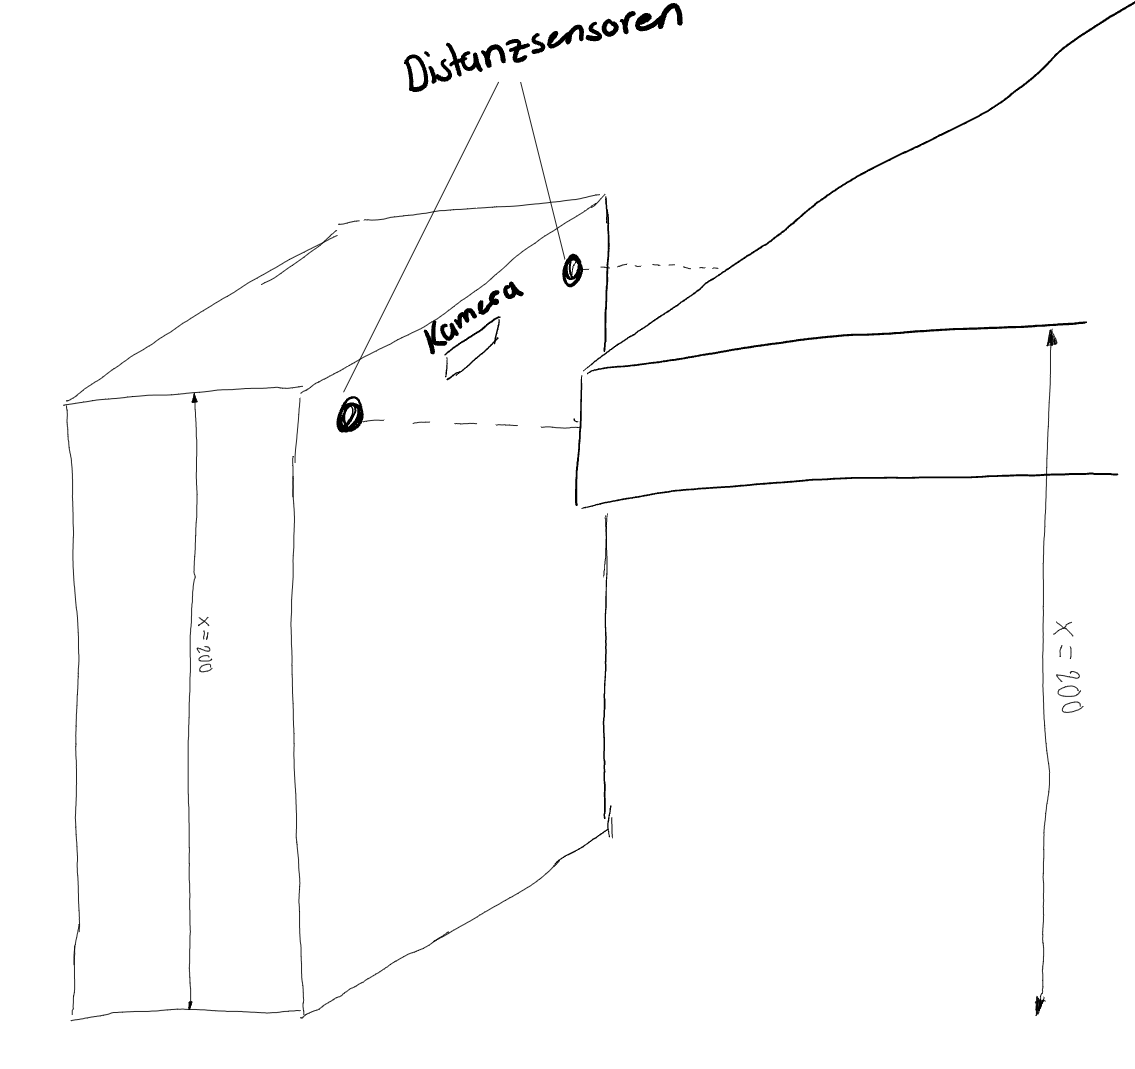
\includegraphics[width=0.7\textwidth]{img/orientierung-treppenstufe/Distanzsensoren.png}
  \centering
  \caption{Skizze der Befestigungspunkte der Distanzsensoren}
  \label{fig:distanzsensoren}
\end{figure}

\subsubsection{Orientierung auf der Treppenstufe}
\label{sec:orientierung-auf-der-treppenstufe}
Um sich auf einer Treppenstufe orientieren zu können, ist geplant mithilfe eines Linefollowing Algorithmus der Treppenstufe sicher entlang zu fahren. Ebenfalls ist gedacht, den Linefollowing Algorithmus dazu zu verwenden, die Ausrichtung des Roboters auf der Treppenstufe zu kontrollieren (siehe Kapitel \ref{sec:orientierung-auf-treppenstufe-funktionsmuster}).
Die zurückgelegte Distanz auf einer Treppenstufe soll mithilfe des Encoders der Motoren berechnet werden.

\subsubsection{Hindernisserkennung}
\label{sec:hindernisserkennung}
Auch bei der Hindernisserkennung wurde versucht eine Lösung zu finden, welche so einfach wie möglich ist.
Einige Ideen wie das Erkennen der Hindernisse mit einem \acrshort{tof} Sensor wurden schnell wieder verworfen,
da man ein Hindernis, welches sich hinter einem anderen Hindernis befindet nicht finden kann.

Die Hindernisse sind gut erkennbar, wenn sie mit einer Raspberry Kamera aus Sicht des Roboters 
fotografiert werden. Aus diesem Grund wurde
auch die Hindernisserkennung mit der Kamera zu realisieren.

Wie in Kapitel \nameref{sec:hindernisserkennung-funktinosmuster} beschrieben, wurden dazu einige Ansätze verfolgt um Aufwand, Komplexität und Rechenleistung zu minimieren nach dem \acrshort{kiss} Prinzip.
Es wurden ein einfacher Farbfilter und Rechteckmarkierung probiert (Siehe Abbildung \ref{fig:color-detection-1}).
Dieser war leider schon bei Optimierung auf die idealen Lichtverhältnisse relativ ungenau.
Ein weiterer Ansatz war, den Informationsgehalt zu minimieren und nur die Treppenstufen auf dem Bild auszuschneiden.
Dies kann natürlich nur unter der Annahme gemacht werden, dass sich der Roboter immer genau an der gleichen Stelle
befindet während die Hindernisse erkennt werden und sich die Konfiguration der Treppe nicht ändert.
Da bereits kleine Abweichungen das Resultat massiv beeinträchtigen können und dass Ziegelsteine, welche
über zwei Treppenstufen hinausragen nicht richtig erkannt werden können, ist auch diese Methode zu ungenau.

\acrfull{cnn} wurden geschaffen um genau solche Objekterkennungsprobleme zu lösen.
Da wir auf dem Raspberry nur beschränkte Rechenleistung haben eignet sich dafür die \acrfull{yolo} CNN 
Architektur \cite{YOLOv3}. Mit dem Tiny-\acrshort{yolo} kann auf einem Raspberry PI, mit genügend input daten, eine
fast Real-Time Objekterkennung realisiert werden \cite{YOLORaspi}.


\subsubsection{Piktogrammerkennung}
\label{piktogrammerkennung}
Erst war geplant, die Piktogrammerkennung mit einem \acrfull{cnn} zu realisieren. Hierbei wird ein Modell darauf trainiert, die fünf Piktogramme zu erkennen. Während der Erstellung des Funktionsmusters (siehe Kapitel \ref{sec:piktogrammerkennung-mit-cnn}) und den Weekly-Standups mit dem Coach hat sich herausgestellt, dass es passendere Techniken gibt.\\
Da es sich um ein endliches Problem handelt, weil man lediglich fünf verschiedene Piktogramme erkennen und unterscheiden muss, war der zweite Lösungsansatz sogenanntes Template Matching \cite{OpenCV-Template-Matching}. Bei der Recherche hat sich herausgestellt, dass diese Methode gute Resultate liefert, wenn man lediglich mit Translationen und Skalierungen zu tun hat. Sobald das Bild, in dem das Piktogramm detektiert werden soll, Rotationen und nicht affine Transformationen aufweist, ist es sinnvoller Keypoint Detection, Image Deskriptoren und Keypoint Matching \cite{OpenCV-Feature-Matching} zu verwenden. Aus diesem Grund ist geplant die Piktogrammerkennung mit letzterem umzusetzen.



\subsection {Kommunikation}
\label{sec:kommunikation}
Um das Finden und Verarbeiten des Piktogramms sowohl im Start- als auch im Zielbereich zuverlässig und einfach zu signalisieren, werden zwei verschiedene Methoden verwendet. Einerseits die Visualisierung mittels LEDs und anderseits die auditive Quittierung. Diese Audiowiedergabe wird entweder mittels Buzzer, oder mittels eines Lautsprechers getätigt. Die Visualisierung mittels LEDs erfolgt über das Raspberry selbst.

Die Audiowiedergabe über den Buzzer ermöglicht einfache Tonabfolgen und wird über die Spannung eines Pins gesteuert. Das Prinzip ist einfach und schnell, ist bezüglich der Lautstärke und dem \glqq WoW-Effekt \grqq{} dem Lautsprecher jedoch deutlich unterlegen.
Die Ausgabe über die USB-Lautsprecher erfolgt direkt über das Raspberry. Die Speaker werden direkt mittels USB und der 3.5mm Klinke mit dem Raspberry verbunden. Mit wenigen Zeilen Code kann so ein vollwertiges Audiofile abgespielt werden.
Die Lautsprecher sind in jeglicher Hinsicht besser und einfacher mit der Ausnahme des Platzbedarfs. Ist der Platz und das Gewicht verfügbar, werden die Lautsprecher verbaut.

\newpage
\subsection{Zusammenspiel der Teilfunktionen}
 Die Abbildung \ref{blockschaltbild} zeigt das Blockschaltbild des Zusammenspiels der Teilfunktionen.

\begin{figure}[h]
  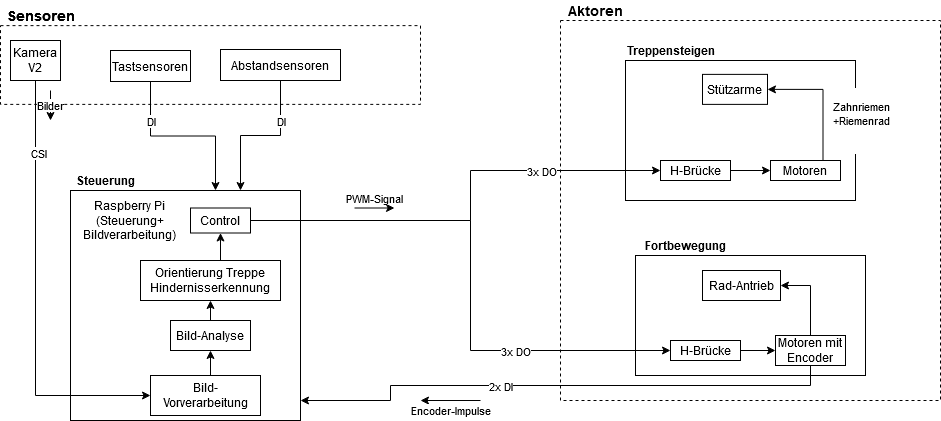
\includegraphics[width=\textwidth]{img/Funktionsmuster Treppensteigen/Blockschaltbild_V2.png}
  \centering
  \caption{Blockschaltbild}
  \label{blockschaltbild}
\end{figure}

 Das Blockschaltbild enthält als zentrale Steuerungseinheit einen Raspberry Pi. Dieser übernimmt die Aufgabe der Bildverarbeitung für die Orientierung auf der Treppe sowie für die Hinderniserkennung. Diese Informationen verarbeitet die Steuerung und gibt entsprechende Signale an die Aktoren weiter. Zu den Aktoren gehören die Elektromotoren inklusive der H-Brücken für die Ansteuerung, sowie die mechanischen Komponenten für das Treppensteigen und die Fortbewegung. Die Elektromotoren der Fortbewegung senden ein Encodersignal zurück an den Raspberry Pi. Zu den Sensoren des Konzeptes gehören Kameras, die Bilder für die Bildverarbeitung liefern. Zusätzlich liefern Abstands- und Tastsensoren für die Orientierung und das Treppensteigen Inputsignale für die Steuerung.

\newpage



\subsection{Schnittstellenbeschreibung}
Die Abbildung \ref{schnittstellen} zeigt die Schnittstellen der Aktoren und Sensoren, welche mit dem Raspberry Pi verbunden sind.

\begin{figure}[h]
  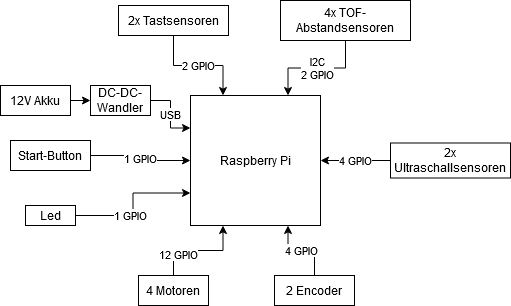
\includegraphics[width=0.65\textwidth]{img/Funktionsmuster Treppensteigen/Schnittstellen.png}
  \centering
  \caption{Schnittstellendiagramm}
  \label{schnittstellen}
\end{figure}

Zu den Schnittstellen gehören die USB-Schnittstelle für die Stromversorgung des Raspberry Pi, die \acrshort{i2c}-Schnittstelle für die \acrshort{tof}-Abstandssensoren, sowie die digitalen \acrfull{gpio} für die Tastsensoren, Ultrasschallsensoren, LED, Start-Taster und die Motoren mit Encoder. Der Raspberry Pi wird mit 5V versorgt werden muss, wird ein DC-DC-Abwärtswandler verwendet, welcher die Spannung des Akkus von 12V auf 5.1V wandelt. Die Versorgungsspannung ist um 0.1V erhöht, um allfällige Schwankungen durch Belastung auszugleichen. Ausserdem versorgt der DC-DC-Wandler die restlichen Sensoren mit Spannung, da die Ausgangsspannung vom Raspberry Pi nicht zu stark belastet werden dürfen.
Der \acrshort{i2c} ist ein simpler serieller Master-Slave-Datenbus, wobei die Datenübertragung über zwei Leitungen erfolgt: eine Datenleitung (SDA) und eine Taktleitung (SCL). Der \acrshort{i2c}-Master (Raspberry Pi) kann bis zu 112 Geräte (Slaves) mit einer 7-Bit-Adresse ansprechen \cite{I2C}. Ein weiterer Vorteil ist, dass es bereits Libraries für die Implementierung der Schnittstelle gibt.

\newpage
\begin{figure}[ht]
 \begin{minipage}{0.5\textwidth}
 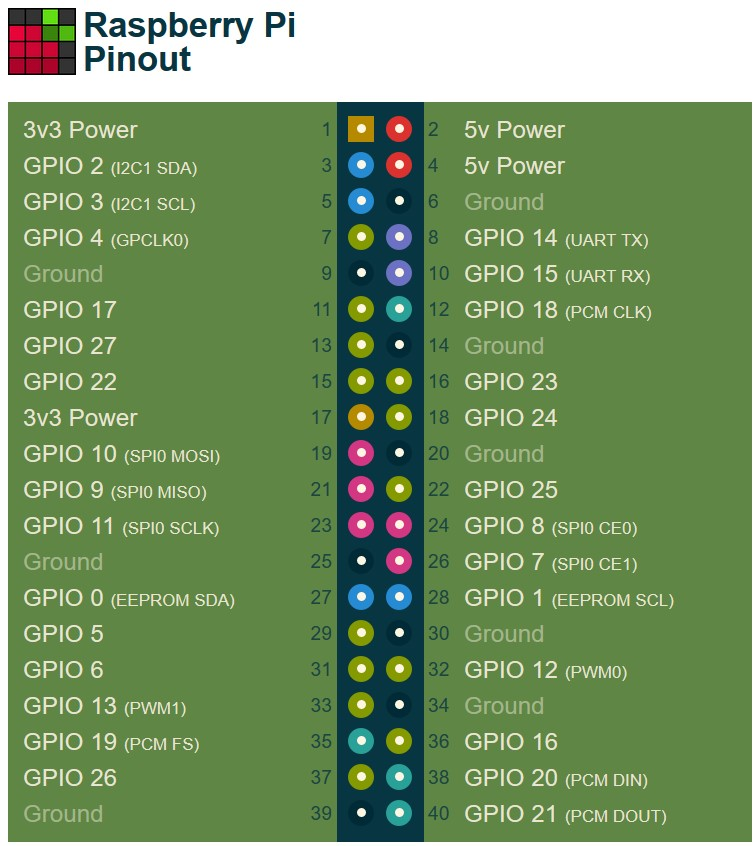
\includegraphics[width=0.9\textwidth]{img/Funktionsmuster Treppensteigen/Pinout.png}
 \caption{Pinbelegung eines Raspberry Pi}
 \end{minipage} 
	\hfill
	\begin{minipage}{0.5\textwidth}
 Die Komponenten benötigen insgesamt 24 \acrshort{gpio}s und an einem Raspberry Pi 3 sind 28 \acrshort{gpio}s verfügbar\footnotemark. Falls die Anzahl Pins im Laufe der Entwicklung nicht ausreicht, besteht die Möglichkeit durch ein Erweiterungsboard mit \acrshort{i2c} die \acrshort{gpio}s zu erweitern.
 \vspace{5cm}
 \end{minipage}
\end{figure}
\footnotetext{https://pinout.xyz/\#}
